%%=============================================================================
%% LaTeX sjabloon voor bachelorproef, HoGent Bedrijf en Organisatie
%% Opleiding Toegepaste Informatica
%%============================================================================


\documentclass[fleqn,a4paper,12pt]{book}


%%=============================================================================
%% LaTeX sjabloon voor de bachelorproef, HoGent Bedrijf en Organisatie
%% Opleiding toegepaste informatica
%%
%% Structuur en algemene vormgeving. Meestal hoef je hier niets te wijzigen.
%%
%% Vormgeving gebaseerd op "The Legrand Orange Book", version 2.0 (9/2/15)
%% door Mathias Legrand (legrand.mathias@gmail.com) met aanpassingen door
%% Vel (vel@latextemplates.com). Het oorspronkelijke template is te vinden op
%% http://www.LaTeXTemplates.com
%%
%% Aanpassingen voor HoGent toegepaste informatica: 
%%   Bert Van Vreckem <bert.vanvreckem@hogent.be>
%% Licentie: 
%%   CC BY-NC-SA 3.0 (http://creativecommons.org/licenses/by-nc-sa/3.0/)
%%=============================================================================

%%-----------------------------------------------------------------------------
%% Packages
%%-----------------------------------------------------------------------------

\usepackage[top=3cm,bottom=3cm,left=3cm,right=3cm,headsep=10pt,a4paper]{geometry} % Page margins
\usepackage[utf8]{inputenc}  % Accenten gebruiken in tekst (vb. é ipv \'e)
\usepackage{amsfonts}        % AMS math packages: extra wiskundige
\usepackage{amsmath}         %   symbolen (o.a. getallen-
\usepackage{amssymb}         %   verzamelingen N, R, Z, Q, etc.)
\usepackage[english,dutch]{babel}    % Taalinstellingen: woordsplitsingen,
                             %  commando's voor speciale karakters
                             %  ("dutch" voor NL)
\usepackage{iflang}
\usepackage{eurosym}         % Euro-symbool €
\usepackage{geometry}
\usepackage{graphicx}        % Invoegen van tekeningen
\graphicspath{{img/}}       % Specifies the directory where pictures are stored
\usepackage{tikz}            % Required for drawing custom shapes
\usepackage[pdftex,bookmarks=true]{hyperref}
                             % PDF krijgt klikbare links & verwijzingen,
                             %  inhoudstafel
\usepackage{enumitem}        % Customize lists
\setlist{nolistsep}         % Reduce spacing between list items
\usepackage{listings}        % Broncode mooi opmaken
\usepackage{multirow}        % Tekst over verschillende cellen in tabellen
\usepackage{rotating}        % Tabellen en figuren roteren

\usepackage{booktabs}        % Required for nicer horizontal rules in tables

\usepackage{xcolor}          % Required for specifying colors by name
\definecolor{maincolor}{RGB}{0,147,208} % Define the main color used for 
                             % highlighting throughout the book
                             % 0, 147, 208 = officiële kleur HoGent FBO

% Paragraph style: no indent, add space between paragraphs
\setlength{\parindent}{0em}
\setlength{\parskip}{1em}

\usepackage{etoolbox}
\usepackage{titling} % Macros for title, author, etc
\usepackage{lipsum}          % Voor vultekst (lorem ipsum)

%----------------------------------------------------------------------------------------
%	FONTS
%----------------------------------------------------------------------------------------

\usepackage{avant} % Use the Avantgarde font for headings
%\usepackage{times} % Use the Times font for headings
\usepackage{mathptmx} % Use the Adobe Times Roman as the default text font together with math symbols from the Sym­bol, Chancery and Com­puter Modern fonts

\usepackage{microtype} % Slightly tweak font spacing for aesthetics
\usepackage[utf8]{inputenc} % Required for including letters with accents
\usepackage[T1]{fontenc} % Use 8-bit encoding that has 256 glyphs

%------------------------------------------------------------------------------
%	TITLE PAGE
%------------------------------------------------------------------------------

\newcommand{\inserttitlepage}{%
\begin{titlepage}
  \newgeometry{top=2cm,bottom=1.5cm,left=1.5cm,right=1.5cm}
  \begin{center}

    \begingroup
    \rmfamily
    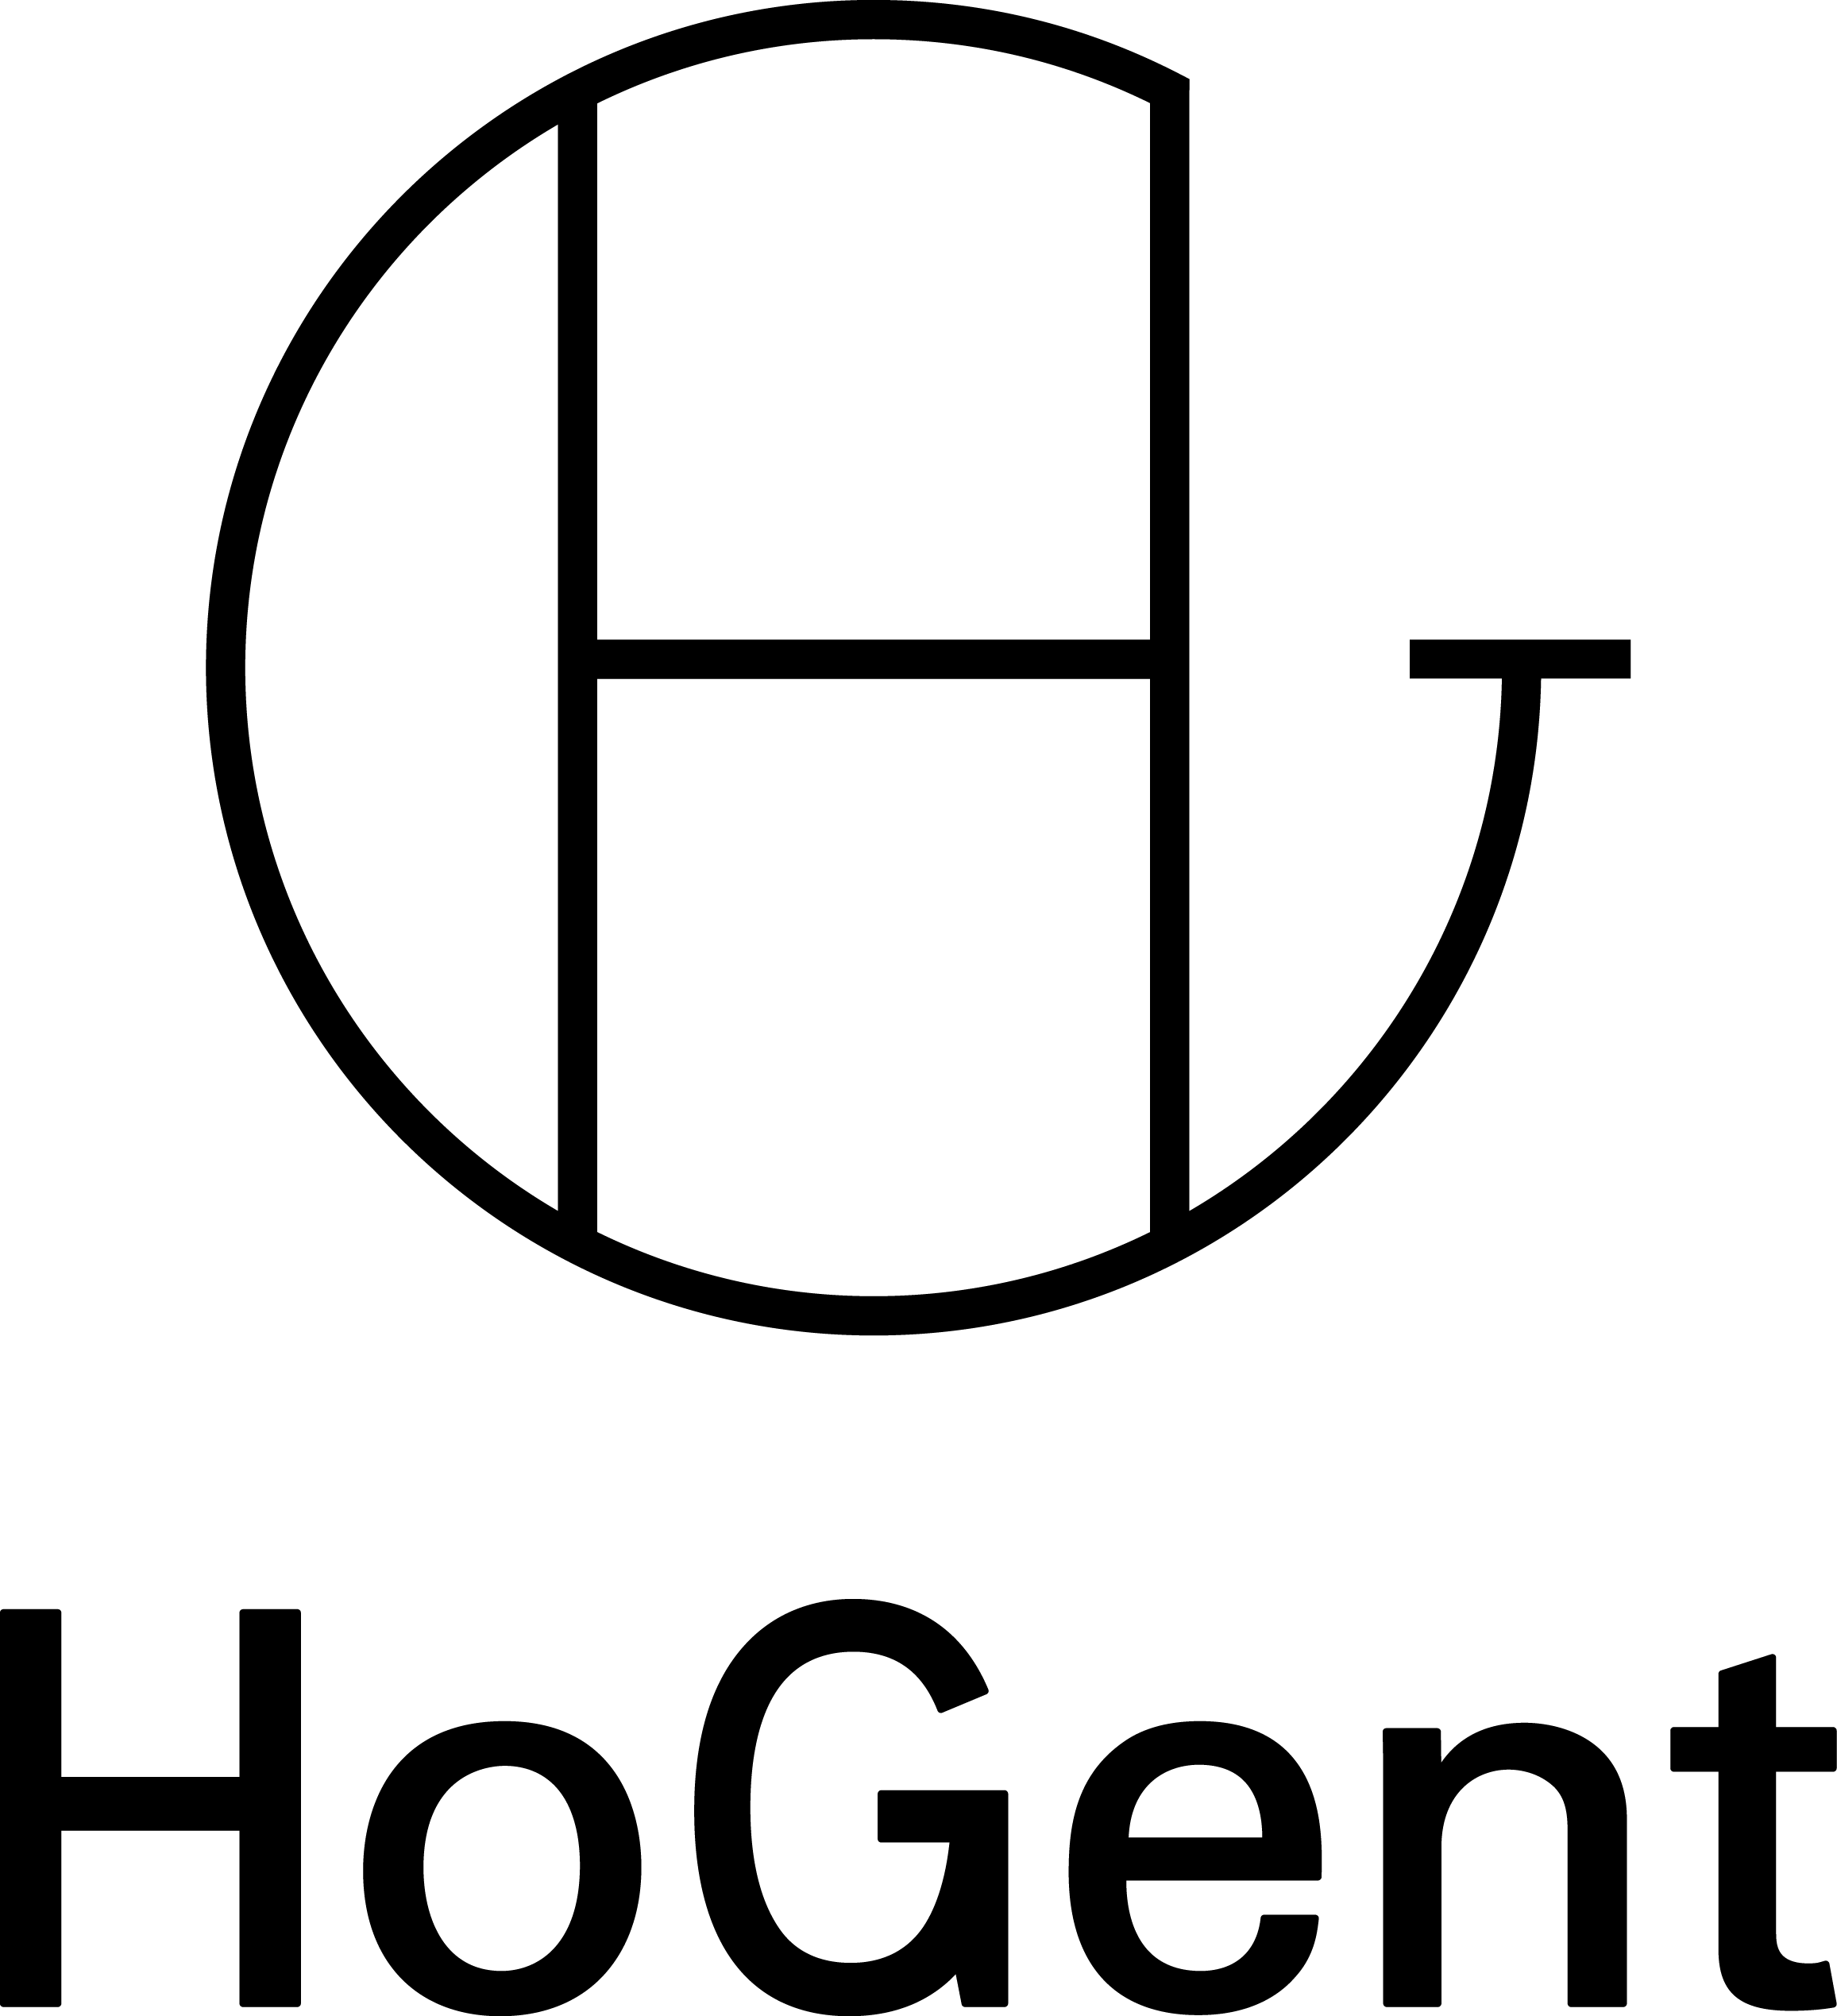
\includegraphics[width=2.5cm]{img/HG-beeldmerk-woordmerk}\\[.5cm]
    Faculteit Bedrijf en Organisatie\\[3cm]
    \titel
    \vfill
    \student\\[3.5cm]
    Scriptie voorgedragen tot het bekomen van de graad van\\professionele bachelor in de toegepaste informatica\\[2cm]
    Promotor:\\
    \promotor\\
    \ifdefempty{\copromotor}{\vspace{2.5cm}}{Co-promotor:\\\copromotor\\[2.5cm]}
    Instelling: \instelling\\[.5cm]
    Academiejaar: \academiejaar\\[.5cm]
    \ifcase \examenperiode \or Eerste \or Tweede \else Derde \fi examenperiode
    \endgroup

  \end{center}
  \restoregeometry
\end{titlepage}
  \emptypage
\begin{titlepage}
  \newgeometry{top=5.35cm,bottom=1.5cm,left=1.5cm,right=1.5cm}
  \begin{center}

    \begingroup
    \rmfamily
    \IfLanguageName{dutch}{Faculteit Bedrijf en Organisatie}{Faculty of Business and Information Management}\\[3cm]
    \titel
    \vfill
    \student\\[3.5cm]
    \IfLanguageName{dutch}{Scriptie voorgedragen tot het bekomen van de graad van\\professionele bachelor in de toegepaste informatica}{Thesis submitted in partial fulfilment of the requirements for the degree of\\professional bachelor of applied computer science}\\[2cm]
    Promotor:\\
    \promotor\\
    \ifdefempty{\copromotor}{\vspace{2.5cm}}{Co-promotor:\\\copromotor\\[2.5cm]}
    \IfLanguageName{dutch}{Instelling}{Institution}: \instelling\\[.5cm]
    \IfLanguageName{dutch}{Academiejaar}{Academic year}: \academiejaar\\[.5cm]
    \IfLanguageName{dutch}{%
    \ifcase \examenperiode \or Eerste \or Tweede \else Derde \fi examenperiode}{%
    \ifcase \examenperiode \or First \or Second \else Third \fi examination period}
    \endgroup

  \end{center}
  \restoregeometry
\end{titlepage}
}

%----------------------------------------------------------------------------------------
%	BIBLIOGRAPHY AND INDEX
%----------------------------------------------------------------------------------------

\usepackage[style=apa,backend=biber]{biblatex}
\usepackage{csquotes}
\DeclareLanguageMapping{dutch}{dutch-apa}
\addbibresource{bachproef-tin.bib} % BibTeX bibliography file
\addbibresource{../voorstel/voorstel.bib}
\defbibheading{bibempty}{}

\usepackage{calc} % For simpler calculation - used for spacing the index letter headings correctly
\usepackage{makeidx} % Required to make an index
\makeindex % Tells LaTeX to create the files required for indexing

%----------------------------------------------------------------------------------------
%	MAIN TABLE OF CONTENTS
%----------------------------------------------------------------------------------------

\usepackage{titletoc} % Required for manipulating the table of contents

\contentsmargin{0cm} % Removes the default margin

% Part text styling
\titlecontents{part}[0cm]
{\addvspace{20pt}\centering\large\bfseries}
{}
{}
{}

% Chapter text styling
\titlecontents{chapter}[1.25cm] % Indentation
{\addvspace{12pt}\large\sffamily\bfseries} % Spacing and font options for chapters
{\color{maincolor!60}\contentslabel[\Large\thecontentslabel]{1.25cm}\color{maincolor}} % Chapter number
{\color{maincolor}}
{\color{maincolor!60}\normalsize\;\titlerule*[.5pc]{.}\;\thecontentspage} % Page number

% Section text styling
\titlecontents{section}[1.25cm] % Indentation
{\addvspace{3pt}\sffamily\bfseries} % Spacing and font options for sections
{\contentslabel[\thecontentslabel]{1.25cm}} % Section number
{}
{\hfill\color{black}\thecontentspage} % Page number
[]

% Subsection text styling
\titlecontents{subsection}[1.25cm] % Indentation
{\addvspace{1pt}\sffamily\small} % Spacing and font options for subsections
{\contentslabel[\thecontentslabel]{1.25cm}} % Subsection number
{}
{\ \titlerule*[.5pc]{.}\;\thecontentspage} % Page number
[]

% List of figures
\titlecontents{figure}[0em]
{\addvspace{-5pt}\sffamily}
{\thecontentslabel\hspace*{1em}}
{}
{\ \titlerule*[.5pc]{.}\;\thecontentspage}
[]

% List of tables
\titlecontents{table}[0em]
{\addvspace{-5pt}\sffamily}
{\thecontentslabel\hspace*{1em}}
{}
{\ \titlerule*[.5pc]{.}\;\thecontentspage}
[]

%----------------------------------------------------------------------------------------
%	MINI TABLE OF CONTENTS IN PART HEADS
%----------------------------------------------------------------------------------------

% Chapter text styling
\titlecontents{lchapter}[0em] % Indenting
{\addvspace{15pt}\large\sffamily\bfseries} % Spacing and font options for chapters
{\color{maincolor}\contentslabel[\Large\thecontentslabel]{1.25cm}\color{maincolor}} % Chapter number
{}
{\color{maincolor}\normalsize\sffamily\bfseries\;\titlerule*[.5pc]{.}\;\thecontentspage} % Page number

% Section text styling
\titlecontents{lsection}[0em] % Indenting
{\sffamily\small} % Spacing and font options for sections
{\contentslabel[\thecontentslabel]{1.25cm}} % Section number
{}
{}

% Subsection text styling
\titlecontents{lsubsection}[.5em] % Indentation
{\normalfont\footnotesize\sffamily} % Font settings
{}
{}
{}

%----------------------------------------------------------------------------------------
%	PAGE HEADERS
%----------------------------------------------------------------------------------------

\usepackage{fancyhdr} % Required for header and footer configuration

\pagestyle{fancy}
\renewcommand{\chaptermark}[1]{\markboth{\sffamily\normalsize\bfseries\chaptername\ \thechapter.\ #1}{}} % Chapter text font settings
\renewcommand{\sectionmark}[1]{\markright{\sffamily\normalsize\thesection\hspace{5pt}#1}{}} % Section text font settings
\fancyhf{} \fancyhead[LE,RO]{\sffamily\normalsize\thepage} % Font setting for the page number in the header
\fancyhead[LO]{\rightmark} % Print the nearest section name on the left side of odd pages
\fancyhead[RE]{\leftmark} % Print the current chapter name on the right side of even pages
\renewcommand{\headrulewidth}{0.5pt} % Width of the rule under the header
\addtolength{\headheight}{2.5pt} % Increase the spacing around the header slightly
\renewcommand{\footrulewidth}{0pt} % Removes the rule in the footer
\fancypagestyle{plain}{\fancyhead{}\renewcommand{\headrulewidth}{0pt}} % Style for when a plain pagestyle is specified

% Removes the header from odd empty pages at the end of chapters
\makeatletter
\renewcommand{\cleardoublepage}{
\clearpage\ifodd\c@page\else
\hbox{}
\vspace*{\fill}
\thispagestyle{empty}
\newpage
\fi}

%----------------------------------------------------------------------------------------
%	THEOREM STYLES
%----------------------------------------------------------------------------------------

\usepackage{amsmath,amsfonts,amssymb,amsthm} % For math equations, theorems, symbols, etc

\newcommand{\intoo}[2]{\mathopen{]}#1\,;#2\mathclose{[}}
\newcommand{\ud}{\mathop{\mathrm{{}d}}\mathopen{}}
\newcommand{\intff}[2]{\mathopen{[}#1\,;#2\mathclose{]}}
\newtheorem{notation}{Notation}[chapter]

% Boxed/framed environments
\newtheoremstyle{maincolornumbox}% % Theorem style name
{0pt}% Space above
{0pt}% Space below
{\normalfont}% % Body font
{}% Indent amount
{\small\bf\sffamily\color{maincolor}}% % Theorem head font
{\;}% Punctuation after theorem head
{0.25em}% Space after theorem head
{\small\sffamily\color{maincolor}\thmname{#1}\nobreakspace\thmnumber{\@ifnotempty{#1}{}\@upn{#2}}% Theorem text (e.g. Theorem 2.1)
\thmnote{\nobreakspace\the\thm@notefont\sffamily\bfseries\color{black}---\nobreakspace#3.}} % Optional theorem note
\renewcommand{\qedsymbol}{$\blacksquare$}% Optional qed square

\newtheoremstyle{blacknumex}% Theorem style name
{5pt}% Space above
{5pt}% Space below
{\normalfont}% Body font
{} % Indent amount
{\small\bf\sffamily}% Theorem head font
{\;}% Punctuation after theorem head
{0.25em}% Space after theorem head
{\small\sffamily{\tiny\ensuremath{\blacksquare}}\nobreakspace\thmname{#1}\nobreakspace\thmnumber{\@ifnotempty{#1}{}\@upn{#2}}% Theorem text (e.g. Theorem 2.1)
\thmnote{\nobreakspace\the\thm@notefont\sffamily\bfseries---\nobreakspace#3.}}% Optional theorem note

\newtheoremstyle{blacknumbox} % Theorem style name
{0pt}% Space above
{0pt}% Space below
{\normalfont}% Body font
{}% Indent amount
{\small\bf\sffamily}% Theorem head font
{\;}% Punctuation after theorem head
{0.25em}% Space after theorem head
{\small\sffamily\thmname{#1}\nobreakspace\thmnumber{\@ifnotempty{#1}{}\@upn{#2}}% Theorem text (e.g. Theorem 2.1)
\thmnote{\nobreakspace\the\thm@notefont\sffamily\bfseries---\nobreakspace#3.}}% Optional theorem note

% Non-boxed/non-framed environments
\newtheoremstyle{maincolornum}% % Theorem style name
{5pt}% Space above
{5pt}% Space below
{\normalfont}% % Body font
{}% Indent amount
{\small\bf\sffamily\color{maincolor}}% % Theorem head font
{\;}% Punctuation after theorem head
{0.25em}% Space after theorem head
{\small\sffamily\color{maincolor}\thmname{#1}\nobreakspace\thmnumber{\@ifnotempty{#1}{}\@upn{#2}}% Theorem text (e.g. Theorem 2.1)
\thmnote{\nobreakspace\the\thm@notefont\sffamily\bfseries\color{black}---\nobreakspace#3.}} % Optional theorem note
\renewcommand{\qedsymbol}{$\blacksquare$}% Optional qed square
\makeatother

% Defines the theorem text style for each type of theorem to one of the three styles above
\newcounter{dummy}
\numberwithin{dummy}{section}
\theoremstyle{maincolornumbox}
\newtheorem{theoremeT}[dummy]{Theorem}
\newtheorem{problem}{Problem}[chapter]
\newtheorem{exerciseT}{Exercise}[chapter]
\theoremstyle{blacknumex}
\newtheorem{exampleT}{Example}[chapter]
\theoremstyle{blacknumbox}
\newtheorem{vocabulary}{Vocabulary}[chapter]
\newtheorem{definitionT}{Definition}[section]
\newtheorem{corollaryT}[dummy]{Corollary}
\theoremstyle{maincolornum}
\newtheorem{proposition}[dummy]{Proposition}

%----------------------------------------------------------------------------------------
%	DEFINITION OF COLORED BOXES
%----------------------------------------------------------------------------------------

\RequirePackage[framemethod=default]{mdframed} % Required for creating the theorem, definition, exercise and corollary boxes

% Theorem box
\newmdenv[skipabove=7pt,
skipbelow=7pt,
backgroundcolor=black!5,
linecolor=maincolor,
innerleftmargin=5pt,
innerrightmargin=5pt,
innertopmargin=5pt,
leftmargin=0cm,
rightmargin=0cm,
innerbottommargin=5pt]{tBox}

% Exercise box
\newmdenv[skipabove=7pt,
skipbelow=7pt,
rightline=false,
leftline=true,
topline=false,
bottomline=false,
backgroundcolor=maincolor!10,
linecolor=maincolor,
innerleftmargin=5pt,
innerrightmargin=5pt,
innertopmargin=5pt,
innerbottommargin=5pt,
leftmargin=0cm,
rightmargin=0cm,
linewidth=4pt]{eBox}

% Definition box
\newmdenv[skipabove=7pt,
skipbelow=7pt,
rightline=false,
leftline=true,
topline=false,
bottomline=false,
linecolor=maincolor,
innerleftmargin=5pt,
innerrightmargin=5pt,
innertopmargin=0pt,
leftmargin=0cm,
rightmargin=0cm,
linewidth=4pt,
innerbottommargin=0pt]{dBox}

% Corollary box
\newmdenv[skipabove=7pt,
skipbelow=7pt,
rightline=false,
leftline=true,
topline=false,
bottomline=false,
linecolor=gray,
backgroundcolor=black!5,
innerleftmargin=5pt,
innerrightmargin=5pt,
innertopmargin=5pt,
leftmargin=0cm,
rightmargin=0cm,
linewidth=4pt,
innerbottommargin=5pt]{cBox}

% Creates an environment for each type of theorem and assigns it a theorem text style from the "Theorem Styles" section above and a colored box from above
\newenvironment{theorem}{\begin{tBox}\begin{theoremeT}}{\end{theoremeT}\end{tBox}}
\newenvironment{exercise}{\begin{eBox}\begin{exerciseT}}{\hfill{\color{maincolor}\tiny\ensuremath{\blacksquare}}\end{exerciseT}\end{eBox}}
\newenvironment{definition}{\begin{dBox}\begin{definitionT}}{\end{definitionT}\end{dBox}}
\newenvironment{example}{\begin{exampleT}}{\hfill{\tiny\ensuremath{\blacksquare}}\end{exampleT}}
\newenvironment{corollary}{\begin{cBox}\begin{corollaryT}}{\end{corollaryT}\end{cBox}}

%----------------------------------------------------------------------------------------
%	REMARK ENVIRONMENT
%----------------------------------------------------------------------------------------

\newenvironment{remark}{\par\vspace{10pt}\small % Vertical white space above the remark and smaller font size
\begin{list}{}{
\leftmargin=35pt % Indentation on the left
\rightmargin=25pt}\item\ignorespaces % Indentation on the right
\makebox[-2.5pt]{\begin{tikzpicture}[overlay]
\node[draw=maincolor!60,line width=1pt,circle,fill=maincolor!25,font=\sffamily\bfseries,inner sep=2pt,outer sep=0pt] at (-15pt,0pt){\textcolor{maincolor}{R}};\end{tikzpicture}} % Orange R in a circle
\advance\baselineskip -1pt}{\end{list}\vskip5pt} % Tighter line spacing and white space after remark

%----------------------------------------------------------------------------------------
%	SECTION NUMBERING IN THE MARGIN
%----------------------------------------------------------------------------------------

\makeatletter
\renewcommand{\@seccntformat}[1]{\llap{\textcolor{maincolor}{\csname the#1\endcsname}\hspace{1em}}}
\renewcommand{\section}{\@startsection{section}{1}{\z@}
{-4ex \@plus -1ex \@minus -.4ex}
{1ex \@plus.2ex }
{\normalfont\large\sffamily\bfseries}}
\renewcommand{\subsection}{\@startsection {subsection}{2}{\z@}
{-3ex \@plus -0.1ex \@minus -.4ex}
{0.5ex \@plus.2ex }
{\normalfont\sffamily\bfseries}}
\renewcommand{\subsubsection}{\@startsection {subsubsection}{3}{\z@}
{-2ex \@plus -0.1ex \@minus -.2ex}
{.2ex \@plus.2ex }
{\normalfont\small\sffamily\bfseries}}
\renewcommand\paragraph{\@startsection{paragraph}{4}{\z@}
{-2ex \@plus-.2ex \@minus .2ex}
{.1ex}
{\normalfont\small\sffamily\bfseries}}

%----------------------------------------------------------------------------------------
%	PART HEADINGS
%----------------------------------------------------------------------------------------

% numbered part in the table of contents
\newcommand{\@mypartnumtocformat}[2]{%
\setlength\fboxsep{0pt}%
\noindent\colorbox{maincolor!20}{\strut\parbox[c][.7cm]{\ecart}{\color{maincolor!70}\Large\sffamily\bfseries\centering#1}}\hskip\esp\colorbox{maincolor!40}{\strut\parbox[c][.7cm]{\linewidth-\ecart-\esp}{\Large\sffamily\centering#2}}}%
%%%%%%%%%%%%%%%%%%%%%%%%%%%%%%%%%%
% unnumbered part in the table of contents
\newcommand{\@myparttocformat}[1]{%
\setlength\fboxsep{0pt}%
\noindent\colorbox{maincolor!40}{\strut\parbox[c][.7cm]{\linewidth}{\Large\sffamily\centering#1}}}%
%%%%%%%%%%%%%%%%%%%%%%%%%%%%%%%%%%
\newlength\esp
\setlength\esp{4pt}
\newlength\ecart
\setlength\ecart{1.2cm-\esp}
\newcommand{\thepartimage}{}%
\newcommand{\partimage}[1]{\renewcommand{\thepartimage}{#1}}%
\def\@part[#1]#2{%
\ifnum \c@secnumdepth >-2\relax%
\refstepcounter{part}%
\addcontentsline{toc}{part}{\texorpdfstring{\protect\@mypartnumtocformat{\thepart}{#1}}{\partname~\thepart\ ---\ #1}}
\else%
\addcontentsline{toc}{part}{\texorpdfstring{\protect\@myparttocformat{#1}}{#1}}%
\fi%
\startcontents%
\markboth{}{}%
{\thispagestyle{empty}%
\begin{tikzpicture}[remember picture,overlay]%
\node at (current page.north west){\begin{tikzpicture}[remember picture,overlay]%
\fill[maincolor!20](0cm,0cm) rectangle (\paperwidth,-\paperheight);
\node[anchor=north] at (4cm,-3.25cm){\color{maincolor!40}\fontsize{220}{100}\sffamily\bfseries\@Roman\c@part};
\node[anchor=south east] at (\paperwidth-1cm,-\paperheight+1cm){\parbox[t][][t]{8.5cm}{
\printcontents{l}{0}{\setcounter{tocdepth}{1}}%
}};
\node[anchor=north east] at (\paperwidth-1.5cm,-3.25cm){\parbox[t][][t]{15cm}{\strut\raggedleft\color{white}\fontsize{30}{30}\sffamily\bfseries#2}};
\end{tikzpicture}};
\end{tikzpicture}}%
\@endpart}
\def\@spart#1{%
\startcontents%
\phantomsection
{\thispagestyle{empty}%
\begin{tikzpicture}[remember picture,overlay]%
\node at (current page.north west){\begin{tikzpicture}[remember picture,overlay]%
\fill[maincolor!20](0cm,0cm) rectangle (\paperwidth,-\paperheight);
\node[anchor=north east] at (\paperwidth-1.5cm,-3.25cm){\parbox[t][][t]{15cm}{\strut\raggedleft\color{white}\fontsize{30}{30}\sffamily\bfseries#1}};
\end{tikzpicture}};
\end{tikzpicture}}
\addcontentsline{toc}{part}{\texorpdfstring{%
\setlength\fboxsep{0pt}%
\noindent\protect\colorbox{maincolor!40}{\strut\protect\parbox[c][.7cm]{\linewidth}{\Large\sffamily\protect\centering #1\quad\mbox{}}}}{#1}}%
\@endpart}
\def\@endpart{\vfil\newpage
\if@twoside
\if@openright
\null
\thispagestyle{empty}%
\newpage
\fi
\fi
\if@tempswa
\twocolumn
\fi}

%----------------------------------------------------------------------------------------
%	CHAPTER HEADINGS
%----------------------------------------------------------------------------------------

% A switch to conditionally include a picture, implemented by  Christian Hupfer
\newif\ifusechapterimage
\usechapterimagetrue
\newcommand{\thechapterimage}{}%
\newcommand{\chapterimage}[1]{\ifusechapterimage\renewcommand{\thechapterimage}{#1}\fi}%
\def\@makechapterhead#1{%
{\parindent \z@ \raggedright \normalfont
\ifnum \c@secnumdepth >\m@ne
\if@mainmatter
\begin{tikzpicture}[remember picture,overlay]
\node at (current page.north west)
{\begin{tikzpicture}[remember picture,overlay]
\node[anchor=north west,inner sep=0pt] at (0,0) {\ifusechapterimage\includegraphics[width=\paperwidth]{\thechapterimage}\fi};
\draw[anchor=west] (\Gm@lmargin,-9cm) node [line width=2pt,rounded corners=15pt,draw=maincolor,fill=white,fill opacity=0.5,inner sep=15pt]{\strut\makebox[22cm]{}};
\draw[anchor=west] (\Gm@lmargin+.3cm,-9cm) node {\huge\sffamily\bfseries\color{black}\thechapter. #1\strut};
\end{tikzpicture}};
\end{tikzpicture}
\else
\begin{tikzpicture}[remember picture,overlay]
\node at (current page.north west)
{\begin{tikzpicture}[remember picture,overlay]
\node[anchor=north west,inner sep=0pt] at (0,0) {\ifusechapterimage\includegraphics[width=\paperwidth]{\thechapterimage}\fi};
\draw[anchor=west] (\Gm@lmargin,-9cm) node [line width=2pt,rounded corners=15pt,draw=maincolor,fill=white,fill opacity=0.5,inner sep=15pt]{\strut\makebox[22cm]{}};
\draw[anchor=west] (\Gm@lmargin+.3cm,-9cm) node {\huge\sffamily\bfseries\color{black}#1\strut};
\end{tikzpicture}};
\end{tikzpicture}
\fi\fi\par\vspace*{270\p@}}}

%-------------------------------------------

\def\@makeschapterhead#1{%
\begin{tikzpicture}[remember picture,overlay]
\node at (current page.north west)
{\begin{tikzpicture}[remember picture,overlay]
\node[anchor=north west,inner sep=0pt] at (0,0) {\ifusechapterimage\includegraphics[width=\paperwidth]{\thechapterimage}\fi};
\draw[anchor=west] (\Gm@lmargin,-9cm) node [line width=2pt,rounded corners=15pt,draw=maincolor,fill=white,fill opacity=0.5,inner sep=15pt]{\strut\makebox[22cm]{}};
\draw[anchor=west] (\Gm@lmargin+.3cm,-9cm) node {\huge\sffamily\bfseries\color{black}#1\strut};
\end{tikzpicture}};
\end{tikzpicture}
\par\vspace*{270\p@}}
\makeatother

%----------------------------------------------------------------------------------------
%	HYPERLINKS IN THE DOCUMENTS
%----------------------------------------------------------------------------------------

\usepackage{hyperref}
\hypersetup{hidelinks,backref=true,pagebackref=true,hyperindex=true,colorlinks=false,breaklinks=true,urlcolor= maincolor,bookmarks=true,bookmarksopen=false,pdftitle={Title},pdfauthor={Author}}
\usepackage{bookmark}
\bookmarksetup{
open,
numbered,
addtohook={%
\ifnum\bookmarkget{level}=0 % chapter
\bookmarksetup{bold}%
\fi
\ifnum\bookmarkget{level}=-1 % part
\bookmarksetup{color=maincolor,bold}%
\fi
}
}

%----------------------------------------------------------------------------------------
%	Java source code
%----------------------------------------------------------------------------------------

% Commando voor invoegen Java-broncodebestanden (dank aan Niels Corneille)
% Gebruik:
%   \codefragment{source/MijnKlasse.java}{Uitleg bij de code}
%
% Je kan dit aanpassen aan de taal die je zelf het meeste gebruikt in je
% bachelorproef.
\newcommand{\codefragment}[2]{ \lstset{%
  language=java,
  breaklines=true,
  float=th,
  caption={#2},
  basicstyle=\scriptsize,
  frame=single,
  extendedchars=\true
}
\lstinputlisting{#1}}

% Leeg blad
\newcommand{\emptypage}{%
\newpage
\thispagestyle{empty}
\mbox{}
\newpage
}


%%---------- Documenteigenschappen --------------------------------------------
%% TODO: Vul dit aan met je eigen info:

% Je eigen naam
\newcommand{\student}{Michiel Leunens}

% De naam van je promotor (lector van de opleiding)
\newcommand{\promotor}{Tom Antjon}

% De naam van je co-promotor. Als je promotor ook je opdrachtgever is en je
% dus ook inhoudelijk begeleidt (en enkel dan!), mag je dit leeg laten.
\newcommand{\copromotor}{Michiel Cuvelier}

% Indien je bachelorproef in opdracht van/in samenwerking met een bedrijf of
% externe organisatie geschreven is, geef je hier de naam. Zoniet laat je dit
% zoals het is.
\newcommand{\instelling}{beSports bvba - Kayzr}

% De titel van het rapport/bachelorproef
\newcommand{\titel}{Monitoring mogelijkheden in NodeJS toepassingen voor feilloos debuggen in 2019}

% Datum van indienen (gebruik telkens de deadline, ook al geef je eerder af)
\newcommand{\datum}{31 mei 2019}

% Academiejaar
\newcommand{\academiejaar}{2018-2019}

% Examenperiode
%  - 1e semester = 1e examenperiode => 1
%  - 2e semester = 2e examenperiode => 2
%  - tweede zit  = 3e examenperiode => 3
\newcommand{\examenperiode}{2}

%%=============================================================================
%% Inhoud document
%%=============================================================================

\begin{document}

%---------- Taalselectie ------------------------------------------------------
% Als je je bachelorproef in het Engels schrijft, haal dan onderstaande regel
% uit commentaar. Let op: de tekst op de voorkaft blijft in het Nederlands, en
% dat is ook de bedoeling!

%\selectlanguage{english}

% Dit dient voor globabel JavaScript opmaak te ondersteunen. Toegevoegd door mezelve.
\lstset{
	aboveskip=0cm,
	stringstyle=\ttfamily,
	showstringspaces = false,
	basicstyle=\scriptsize\ttfamily,
	commentstyle=\color{gray!45},
	keywordstyle=\bfseries,
	ndkeywordstyle=\bfseries,
	identifierstyle=\ttfamily,
	numbers=left,
	numbersep=15pt,
	numberstyle=\tiny,
	numberfirstline = false,
	breaklines=true
}

\lstdefinelanguage{JavaScript}{
	keywords={typeof, new, true, false, catch, function, return, null, catch, switch, var, const, let, async, await, if, in, while, do, else, case, break, from},
	ndkeywords={class, export, boolean, throw, implements, import, this},
	sensitive=false,
	comment=[l]{//},
	morecomment=[s]{/*}{*/},
	morestring=[b]',
	morestring=[b]"
}

%---------- Titelblad ---------------------------------------------------------
\inserttitlepage

%---------- Samenvatting, voorwoord -------------------------------------------
\usechapterimagefalse
%%=============================================================================
%% Voorwoord
%%=============================================================================

\chapter*{Woord vooraf}
\label{ch:voorwoord}

%% TODO:
%% Het voorwoord is het enige deel van de bachelorproef waar je vanuit je
%% eigen standpunt (``ik-vorm'') mag schrijven. Je kan hier bv. motiveren
%% waarom jij het onderwerp wil bespreken.
%% Vergeet ook niet te bedanken wie je geholpen/gesteund/... heeft

Backend debug-toepassingen zijn vaak slecht onderhouden, incompleet of gewoonweg verschrikkelijk duur. Daarom is deze bachelorproef gemaakt met als doel een open-source debug tool te schenken aan iedereen die een project in Node.js en Express ontwikkelt. Mede mogelijk gemaakt dankzij Kayzr, is het de bedoeling om deze tool online te zetten zodat deze effectief in de praktijk gebruikt kan worden. 

Graag bedank ik meneer Tom Antjon, voor zijn altijd paraat staan, snel mijn vragen te willen beantwoorden en mij een goed inzicht te geven in het werk dat nog gedaan moest worden.

Ook wil ik Kayzr bedanken, voor een onvergetelijke stage, waar mijn vaardigheden als developer \textit{en} als fotograaf enorm hebben kunnen groeien. Zonder hen had ik nooit deze bachelorproef kunnen verwezenlijken. De vrijheid die ik hier kreeg, apprecieerde ik dan ook ten zeerste. Maar, dat zou vooral niet gelukt zijn zonder de hulp van mijn copromotor, Michiel Cuvelier, aan wie ik honderden technische vragen kon stellen en die hij stuk voor stuk uitvoerig beantwoordde. 

Het voelt enorm overweldigend aan  om een eerste open-source tool gepubliceerd te hebben op npm en Github. Ik ben dan ook zeer trots op het resultaat, en hoop dat ik met de hulp van andere ontwikkelaars deze tool verder kan blijven ontwikkelen waardoor meerdere gebruikers hier gebruik van zouden kunnen maken. 

Als laatste wil ik ook mijn vader bedanken voor zijn taal-en communicatieadvies.


%%=============================================================================
%% Samenvatting
%%=============================================================================

% TODO: De "abstract" of samenvatting is een kernachtige (~ 1 blz. voor een
% thesis) synthese van het document.
%
% Deze aspecten moeten zeker aan bod komen:
% - Context: waarom is dit werk belangrijk?
% - Nood: waarom moest dit onderzocht worden?
% - Taak: wat heb je precies gedaan?
% - Object: wat staat in dit document geschreven?
% - Resultaat: wat was het resultaat?
% - Conclusie: wat is/zijn de belangrijkste conclusie(s)?
% - Perspectief: blijven er nog vragen open die in de toekomst nog kunnen
%    onderzocht worden? Wat is een mogelijk vervolg voor jouw onderzoek?
%
% LET OP! Een samenvatting is GEEN voorwoord!

%%---------- Nederlandse samenvatting -----------------------------------------
%
% TODO: Als je je bachelorproef in het Engels schrijft, moet je eerst een
% Nederlandse samenvatting invoegen. Haal daarvoor onderstaande code uit
% commentaar.
% Wie zijn bachelorproef in het Nederlands schrijft, kan dit negeren, de inhoud
% wordt niet in het document ingevoegd.

\IfLanguageName{english}{%
\selectlanguage{dutch}
\chapter*{Samenvatting}
\lipsum[1-4]
\selectlanguage{english}
}{}

%%---------- Samenvatting -----------------------------------------------------
% De samenvatting in de hoofdtaal van het document

\chapter*{\IfLanguageName{dutch}{Samenvatting}{Abstract}}

Dit onderzoek wordt gebruikt om te kijken of er goede methodieken en/of betere alternatieven zijn om processen te debuggen van Node.js en Express applicaties in 2019. Dit werk is in opdracht van het bedrijf Kayzr, dat nood heeft aan een verbeterd debug-proces. Met een beperkt budget zijn bestaande tools ofwel onbetaalbaar, ofwel veel te primitief, en zou er onderzoek moeten gedaan worden aan een goed alternatief dat het beste van beide werelden combineert. Namelijk een betaalbaar pakket dat minimum moet voldoen aan een specifiek aantal functionaliteiten.

In deze proef wordt er onderzoek gedaan naar het ecosysteem van de huidige Javascript scène, en uitleg verschaft over diens meest populaire framework \textit{Node.js}. De vereisten van Kayzr worden geanalyseerd en er zal gekeken worden hoe dit kan opgelost worden met huidige hulpmiddelen en software. Vervolgens zal er een stuk software geschreven worden dat Kayzr's problematiek moet oplossen, waarna deze zal getoetst worden aan de praktijk.

 Het resultaat werd positief ontvangen en werd meteen in de productieomgeving gezet. De software kon ook worden geabstraheerd waardoor het mogelijk werd deze tool te delen met het wereldwijde web. Hierdoor kunnen andere bedrijven en ontwikkelaars hier ook van gebruik maken. De zelfgeschreven tool voldeed aan alle vereisten en er werden zelfs extra functionaliteiten toegevoegd.
 
 Er kan geconcludeerd worden dat de productiesnelheid van Kayzr omhoog is gegaan, de efficiëntie van het debuggen is verbeterd en kostprijs niet is gestegen. Mede dankzij de open source natuur van de tool, kan deze tool verder onderzocht worden om te bekijken of deze nog uitgebreid kan worden met nieuwe functionaliteiten of de huidige verbeterd en geoptimaliseerd kunnen worden. Ook kan er nog gekeken worden of de hoge kostprijs van betalende oplossingen verantwoord is door ze te vergelijken met deze gratis tool, en ook of de tool kan gebruikt worden in bedrijven met een ander businessplan dan Kayzr. Als laatste kan er altijd gekeken worden of er nog betere debug-procesmiddelen bestaan aangezien het ecosysteem van het internet verandert met de dag. 



%---------- Inhoudstafel ------------------------------------------------------
\pagestyle{empty} % No headers
\tableofcontents % Print the table of contents itself
\cleardoublepage % Forces the first chapter to start on an odd page so it's on the right
\pagestyle{fancy} % Print headers again

%---------- Lijst figuren, afkortingen, ... -----------------------------------

% Indien gewenst kan je hier een lijst van figuren/tabellen opgeven. Geef in
% dat geval je figuren/tabellen altijd een korte beschrijving:
%
%  \caption[korte beschrijving]{uitgebreide beschrijving}

\listoffigures
\listoftables

% Als je een lijst van afkortingen of termen wil toevoegen, dan hoort die
% hier thuis. Gebruik bijvoorbeeld de ``glossaries'' package.
% https://www.sharelatex.com/learn/Glossaries

%%---------- Kern -------------------------------------------------------------

%%=============================================================================
%% Inleiding
%%=============================================================================

\chapter{Inleiding}
\label{ch:inleiding}

%De inleiding moet de lezer net genoeg informatie verschaffen om het onderwerp te begrijpen en in te zien waarom de onderzoeksvraag de moeite waard is om te onderzoeken. In de inleiding ga je literatuurverwijzingen beperken, zodat de tekst vlot leesbaar blijft. Je kan de inleiding verder onderverdelen in secties als dit de tekst verduidelijkt. Zaken die aan bod kunnen komen in de inleiding~\autocite{Pollefliet2011}:
%
%\begin{itemize}
%  \item context, achtergrond
%  \item afbakenen van het onderwerp
%  \item verantwoording van het onderwerp, methodologie
%  \item probleemstelling
%  \item onderzoeksdoelstelling
%  \item onderzoeksvraag
%  \item \ldots
%\end{itemize}

\section{Probleemstelling}
\label{sec:probleemstelling}

%Uit je probleemstelling moet duidelijk zijn dat je onderzoek een meerwaarde heeft voor een concrete doelgroep. De doelgroep moet goed gedefinieerd en afgelijnd zijn. Doelgroepen als ``bedrijven,'' ``KMO's,'' systeembeheerders, enz.~zijn nog te vaag. Als je een lijstje kan maken van de personen/organisaties die een meerwaarde zullen vinden in deze bachelorproef (dit is eigenlijk je steekproefkader), dan is dat een indicatie dat de doelgroep goed gedefinieerd is. Dit kan een enkel bedrijf zijn of zelfs één persoon (je co-promotor/opdrachtgever).

Het zoeken naar fouten in software kan een frustrerend, hectisch en vermoeiend proces zijn. Daarom zijn toepassingen die dat proces voor de ontwikkelaar kunnen automatiseren of beter analyseren altijd welkom. Kayzr, een Belgische start-up die zich bezighoudt met het mainstream maken en het organiseren van E-Sports in de Benelux, wenst zulke software zodat hun huidige productieproces versneld kan worden. 
Het concrete probleem van Kayzr is dat zijn processen op verschillende plekken worden gemonitord. De tools zijn incompleet, en daardoor krijgt men een gefragmenteerde collectie aan logs, foutmeldingen, informatie, enzovoort.  Per API call moet men foutmeldingen controleren in de terminal, IP-adressen opzoeken in het Google Cloud platform en andere nuttige informatie staat dan weer eens ergens anders opgeslagen. Hierdoor duurt het lang om fouten te analyseren en tot een mogelijke oplossing te komen. Een degelijke tool zoals PM2, een monitoringtoepassing met veel meer functionaliteiten, meer dan dat Kayzr nodig heeft, vormt meteen een kost die ze niet kunnen verantwoorden. Aan \euro 50 per server per maand, loopt het budget voor een vijftigtal servers te hoog op. Deze kostprijs zou schalen zeer moeilijk of zelfs onmogelijk maken.

\section{Onderzoeksvraag}
\label{sec:onderzoeksvraag}

%Wees zo concreet mogelijk bij het formuleren van je onderzoeksvraag. Een onderzoeksvraag is trouwens iets waar nog niemand op dit moment een antwoord heeft (voor zover je kan nagaan). Het opzoeken van bestaande informatie (bv. ``welke tools bestaan er voor deze toepassing?'') is dus geen onderzoeksvraag. Je kan de onderzoeksvraag verder specifiëren in deelvragen. Bv.~als je onderzoek gaat over performantiemetingen, dan 
De onderzoeksvraag is dus als volgt: bestaat er een mogelijkheid om de monitoringtechnieken van Kayzr, en mogelijk nog andere bedrijven, op een goedkope manier te stroomlijnen en te verbeteren binnen een Node.js omgeving, zodat hun debugproces geoptimaliseerd kan worden? 


\section{Onderzoeksdoelstelling}
\label{sec:onderzoeksdoelstelling}

%Wat is het beoogde resultaat van je bachelorproef? Wat zijn de criteria voor succes? Beschrijf die zo concreet mogelijk.
Het onderzoek is geslaagd wanneer Kayzr tevreden is met de toepassing en er in zijn project gebruik van gaat maken. De gemiddelde tijd om een probleem op te lossen moet dalen en het proces moet efficiënter verlopen. De data die per proces worden verzameld moeten op een goede manier kunnen gevisualiseerd worden zodat deze ook voor andere doeleinden kunnen worden gehanteerd. Er moeten meer data ontleed kunnen worden dan ervoor, en de software moet voldoen aan alle \hyperref[sec:requirements]{opgesomde requirements.}


\section{Opzet van deze bachelorproef}
\label{sec:opzet-bachelorproef}

% Het is gebruikelijk aan het einde van de inleiding een overzicht te
% geven van de opbouw van de rest van de tekst. Deze sectie bevat al een aanzet
% die je kan aanvullen/aanpassen in functie van je eigen tekst.

Verder in dit document bevinden zich de volgende onderdelen:

In Hoofdstuk~\ref{ch:stand-van-zaken} volgt een stand van zaken over JavaScript, Node.js, Express en Express middleware. Ook wordt er onderzoek gedaan naar verschillende monitoringsoftware en middleware die relevant zijn in 2019.

Erna wordt het huidige debug proces bestudeerd in hoofdstuk \ref{ch:kayzrsProblem}. Hoe verloopt dit? Wat kan er beter? Wat kan er sneller? Welke functies moet de nieuwe toepassing bevatten?

Hoofdstuk \ref{ch:methodologie} omvat de strategie van dit onderzoek. Hier wordt er kort uitgelegd dat, op basis van de stand van zaken, tools zijn bestudeerd en samen met de probleemstelling een proof-of-concept zal uitgewerkt worden om te voldoen aan de vraag van Kayzr.

In Hoofdstuk~\ref{ch:proofOfConcept} wordt de software geschreven volgens de requirements van Kayzr. Vervolgens wordt er nagegaan of die software daaraan voldoet, en kan er worden vergeleken met de oude processen.

In Hoofdstuk~\ref{ch:conclusie} wordt er gekeken of er een oplossing bestaat op deze onderzoeksvragen. We kijken of Kayzr deze gaat gebruiken naar de toekomst toe en wat er gaat gebeuren met het eigendom van dit softwareproject.


\chapter{Stand van zaken}
\label{ch:stand-van-zaken}

% Tip: Begin elk hoofdstuk met een paragraaf inleiding die beschrijft hoe
% dit hoofdstuk past binnen het geheel van de bachelorproef. Geef in het
% bijzonder aan wat de link is met het vorige en volgende hoofdstuk.

% Pas na deze inleidende paragraaf komt de eerste sectiehoofding.
%
%Dit hoofdstuk bevat je literatuurstudie. De inhoud gaat verder op de inleiding, maar zal het onderwerp van de bachelorproef *diepgaand* uitspitten. De bedoeling is dat de lezer na lezing van dit hoofdstuk helemaal op de hoogte is van de huidige stand van zaken (state-of-the-art) in het onderzoeksdomein. Iemand die niet vertrouwd is met het onderwerp, weet er nu voldoende om de rest van het verhaal te kunnen volgen, zonder dat die er nog andere informatie moet over opzoeken \autocite{Pollefliet2011}.
%
%Je verwijst bij elke bewering die je doet, vakterm die je introduceert, enz. naar je bronnen. In \LaTeX{} kan dat met het commando \texttt{$\backslash${textcite\{\}}} of \texttt{$\backslash${autocite\{\}}}. Als argument van het commando geef je de ``sleutel'' van een ``record'' in een bibliografische databank in het Bib\TeX{}-formaat (een tekstbestand). Als je expliciet naar de auteur verwijst in de zin, gebruik je \texttt{$\backslash${}textcite\{\}}.
%Soms wil je de auteur niet expliciet vernoemen, dan gebruik je \texttt{$\backslash${}autocite\{\}}. In de volgende paragraaf een voorbeeld van elk.
%
%\textcite{Knuth1998} schreef een van de standaardwerken over sorteer- en zoekalgoritmen. Experten zijn het erover eens dat cloud computing een interessante opportuniteit vormen, zowel voor gebruikers als voor dienstverleners op vlak van informatietechnologie~\autocite{Creeger2009}.

%	EFFECTIEVE LITERATUURSTUDIE

Dit hoofdstuk bestaat uit een zeer uitgebreide literatuurstudie, waarin de kern van het probleem wordt opgesplitst in verschillende delen. In het eerste deel wordt er uitleg gegeven over JavaScript zelf en diens evolutie. Vervolgens volgt er een groot deel over de frameworks Node.js en Express, erna bekijken we het belang van testen en monitoren van software en breiden we uit naar een analyse van zulke monitoringssoftware. In het tweede deel wordt er onderzoek gedaan naar de vraag van Kayzr. Wat wordt er verwacht, welk inzicht moet er gegeven worden, welke features moeten worden uitgewerkt. 

\section{Javascript}
\label{sec:javascript}
Javascript is een programmeertaal gemaakt voor het web, waarmee u statische webpagina's kan omzetten naar dynamische en interactieve websites. Doordat het een enorm krachtige scripttaal is dat speciaal werd ontwikkeld om de functionaliteiten van een doorsnee HTML/CSS-pagina uit te breiden, wordt het bijna onmogelijk om nog iets in te beelden dat niet geïmplementeerd kan worden m.b.v. Javascript. De taal is weakly-typed, functioneel, event-driven en dynamisch. JavaScript bevat een bibliotheek van standaardobjecten samen met specifieke taalelementen zoals operatoren, controlestructuren, enz... Deze kern of 'core' kan makkelijk uitgebreid worden met extra objecten waardoor men JavaScript makkelijk kan specifieren als \textit{Client-side JavaScript} en \textit{Server-side JavaScript}. Client-side JavaScript wordt bijvoorbeeld gebruikt om mooi, visueel, de toeters en bellen van de website mooi te maken, of om te reageren op muiskliks, en nog veel meer. Server-side JavaScript houdt zich eerder bezig met het achterliggende van een site, bijvoorbeeld om een webapplicatie te doen communiceren met een databank. Een zeer bekende en veel gebruikte Server-side JavaScript variant is Node.js, waarover later meer uitleg wordt gegeven. \autocite{Javascript2019}

\subsection{Tijdlijn van JavaScript}
\label{sec:jsTimeline}

Javascript heeft echter een hele evolutie achter de rug. Ontstaan in mei 1995, wordt de taal na vele updates nog steeds dagdagelijks gebruikt en kan het wereldwijde web niet meer ingebeeld worden zonder. Brendan Eich, de auteur van de taal, werkte in 1995 samen met Netscape Communications, de makers van de eerste grote webbrowser genaamd Netscape Navigator, om een taal te implementeren in hun browser waar webontwikkelaars gebruik van zouden kunnen maken. Java, een zeer zware programmeertaal met tal van functionaliteiten was de eerste keuze van Netscape, maar Eich schreef uiteindelijk zijn eigen idee uit van een scripttaal in nog geen 10 dagen en overtuigde Netscape om de lichte, schaalbare en Java-complementerende-taal te adopteren \autocite{Rangpariya2019}. Javascript, toen onder de naam Mocha en vervolgens LiveScript, was geboren en zette de wereld van webontwikkelaars op zijn kop.

Netscape bracht nieuwere versies van JavaScript uit, maar Microsoft dreigde die te onttronen. Niet zoveel later, bracht Microsoft Internet Explorer 3 uit met een eigen variant op Javascript, namelijk JScript. Dit was een zware slag voor Netscape, aangezien Microsoft hen hierdoor zou voorbijsteken, maar was wel een grote stap in de evolutie van JavaScript zoals wij het nu kennen. Dit bracht echter problemen met zich mee, want bedrijven zouden telkens eigen versies van JavaScript uitbrengen wat voor veel compatibiliteitproblemen zou zorgen. Uiteindelijk, in 1997, werd JavaScript 1.1 gestandaardiseerd dankzij het European Computer Manufacturers Association en werd omgedoopt tot ECMAScript. \autocite{Wiley2016} Deze standaard, namelijk ES1 (versie 1), zou dan vertakkingen verhelpen. Implementaties van ECMAScript, waaronder JScript, ActionScript, maar dus ook JavaScript zelf, zouden dan telkens ECMAScript implementeren waardoor de core van de varianten telkens hetzelfde blijft. Nu, in 2019; is JavaScript nog steeds enorm populair en implementeert ondertussen al de 9e versie van ECMAScript: ES2018. Sinds es5 is ECMASCRIPT overgeschakeld naar jaarlijkse releases, startend vanaf ES2015.

\subsection{Waarom JavaScript?}
\label{sec:jsWhy}

JavaScript is niets voor niets enorm populair, zelfs nog steeds na al die jaren, dankzij de vele voordelen dat de taal met zich meebrengt. En die lijst van voordelen wordt per iteratie alleen maar groter. Hieronder worden er enkele kernvoordelen opgesomd.

\subsubsection{Dynamisch}
\label{sec:dynamic}

Een dynamisch getypeerde taal slaat neer op het feit dat het type van waarden kunnen veranderen tijdens uitvoertijd. Dit betekent bijvoorbeeld dat een variable string plots kan gebruikt worden om een som te maken met een getal. Dit maakt uitvoertijd en compileertijd aanzienlijk sneller doordat er niet voortdurend controles moeten plaatsvinden. 

\subsubsection{DOM-manipulatie}
\label{sec:DOM}
\begin{figure}
	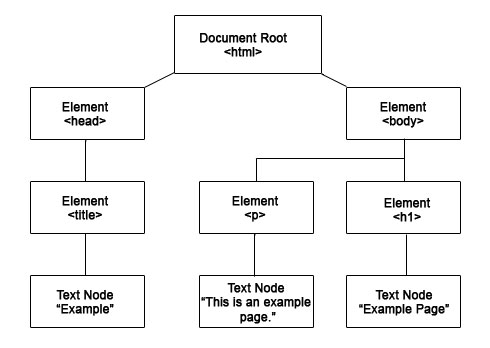
\includegraphics[width=\linewidth]{dom.jpg}
	\caption{Voorbeeld van een DOM structuur.}
	\label{fig:dom}
\end{figure}

De DOM, ofwel Document Object Model, is kortweg het skelet van een HTML-pagina. De structuur van het skelet beschrijft een boomstructuur, waardoor een element een ouder, broer, kind, kleinkind, achterkleinkind, enz... van een element kan zijn. Het HTML element is de wortel van de boom. Client-side JavaScript wordt grotendeels gebruikt om deze boomstructuur te manipuleren. Hierdoor kunnen we HTML elementen toevoegen, verwijderen, stijlen manipuleren, enz... allemaal tijdens uitvoertijd. \textcite{Kantor2017}

\subsubsection{Prototype-based}
\label{sec:prototypeBased}

In JavaScript kan een object eigenlijk aanzien worden als een Array. Hierdoor kunnen ze heel gemakkelijk aan de eigenschappen van een object aan en kunnen we deze ook makkelijk tijdens uitvoertijd aanpassen. Ook kunnen we op deze manier makkelijk eigenschappen aan bestaande objecten toevoegen. In JavaScript wordt gebruikt van de 'dot-notatie' of van de 'haakjesnotatie'. 

	\begin{verbatim}
	foo.bar = 10;
	foo['bar'] = 10;
	const bar = foo.bar;
	foo['bar2'] = bar;
	\end{verbatim}

\subsubsection{Event-driven}
\label{sec:eventDriven}

JavaScript is event-driven, wat betekent dat de code vooral kijkt naar acties van de gebruiker. Bijvoorbeeld: Wanneer een gebruiker op een knop klikt, wil je dat met een animatie de knop heeen en weer beweegt, tekst op je scherm verschijnt, en een server-request wordt gestuurd. 

\subsubsection{Functioneel}
\label{sec:functional}

Sinds ES2015 is JavaScript niet enkel en alleen een object-georiënteerde taal, maar ook een functionele taal. JavaScript was zeer snel met het introduceren van functioneel programmeren (waaronder de populaire arrow-functions). Dit vergemakkelijkte de taal aanzienlijker, aangezien veel minder code geschreven moest worden om hetzelfde resultaat te bereiken.

\subsubsection{Universeel}
\label{sec:universal}

JavaScript wordt sinds ES5 ondersteund door alle moderne browsers! Of er nu in Chrome, Firefox, Safari, Edge of het oude Internet Explorer\footnote{Internet Explorer wordt niet meer verder ontwikkelt, dus ondersteunt het enkel ES2015.} wordt gesurft, ze ondersteunen allemaal JavaScript. D.m.v. de console in de browser te openen kan er al geprogrammeerd worden.





\section{Node.js}
\label{sec:nodeJs}

Node.js is een JavaScript runtime omgeving dat wordt gebruikt voor Server-side toepassingen. Node.js maakt het mogelijk, (of eerder \textit{makkelijker}), om JavaScript nu ook te gebruiken buiten websites maken. Aangezien JavaScript zo'n krachtige taal is, hadden de ontwikkelaars van Node.js een ding in gedachten: JavaScript niet enkel in de browsers, maar ook als alleenstaande applicatie. JavaScript sindsdien evenaren aan andere scripttalen, zoals Python. \textcite{Patel2018}

\subsection{Tijdlijn van Node.js}
\label{sec:nodeTimeline}
Node.js' verhaal start in 2009, toen een ontwikkelaar genaamd Ryan Dahl het niet zo goed stelde met Apache Http Servers. 

Zoals beschreven in \autocite{Chaniotis2015}, was (en is in grote mate nog steeds) Apache HTTP, in combinatie met PHP, jarenlang de go-to-taal om webapplicaties te laten communiceren met databases en server-side functionaliteiten toe te voegen aan webapplicaties, zoals authenticatie, file-en-ftpservers, logging en nog veel meer. PHP is echter nooit in het achterhoofd ontwikkelt geweest om hedendaagse, complexe webapplicaties te schrijven. Ten tweede was Apache incapabel om te schalen naar meerdere processorkernen, waardoor de performantie enorm daalde. PHP in combinatie met Apache was gewoonweg niet gemaakt voor de volgende generatie webapplicaties. Andere struikelblokken zijn cross-platform mobiele applicaties en real-time communicatie.

Meer en meer applicaties worden gemaakt met cross-platform compatibiliteit in het achterhoofd, aangezien de toestroming van verschillende nieuwe besturingssystemen en apparaten het meer en meer onmogelijk maken om native apps\footnote{Native Apps zijn applicaties die gemaakt worden met één besturingssysteem in het hoofd. Bv: Android, IOS.} te ontwikkelen. Hierdoor worden bibliotheken en frameworks ontwikkelt zoals React Native, Flutter, Xamarin, Ionic, PhoneGap, enz... die deze nadelen kunnen overbruggen. Deze zijn echter zo krachtig geworden en schenken zoveel nieuwe voordelen, dat server-side talen en frameworks zoals Apache HTTP/PHP eerder een bottleneck vormden. 

Real-time communicatie is nog een factor dat niet ondersteunt wordt door Apache. Apache was niet ontwikkelt om berichten te sturen naar de client-side. In de wereld van vandaag, waarin sociale media nog nooit zo'n grote invloed heeft gehad op ons dagelijks leven, is het haast ondenkbaar dat real-time communicatie niet zou kunnen bestaan. 

Dit alles zorgde voor de ontwikkeling van Node.js. Dahl's project werd met open armen ontvangen. Na enkele struikelblokken, kende Node.js in 2011 voor het eerst het licht en wordt nu zo'n tien jaar later, gebruikt in vele moderne applicaties en is nog steeds één van de meest begeerde vaardigheden van een programmeur. \autocite{Patel2018}

Hoewel Apache en PHP nog steeds overduidelijk op plaats één staan, hebben ze hun populariteit enkel nog te danken aan bedrijven die op verouderde software werken, en hun populariteit bij senior ontwikkelaars. PHP blijft een geliefde taal bij velen, maar we zien dat Node.js populariteit duidelijk die van Apache aan het inhalen is. \autocite{SimilarTech}

\begin{figure}[h]
	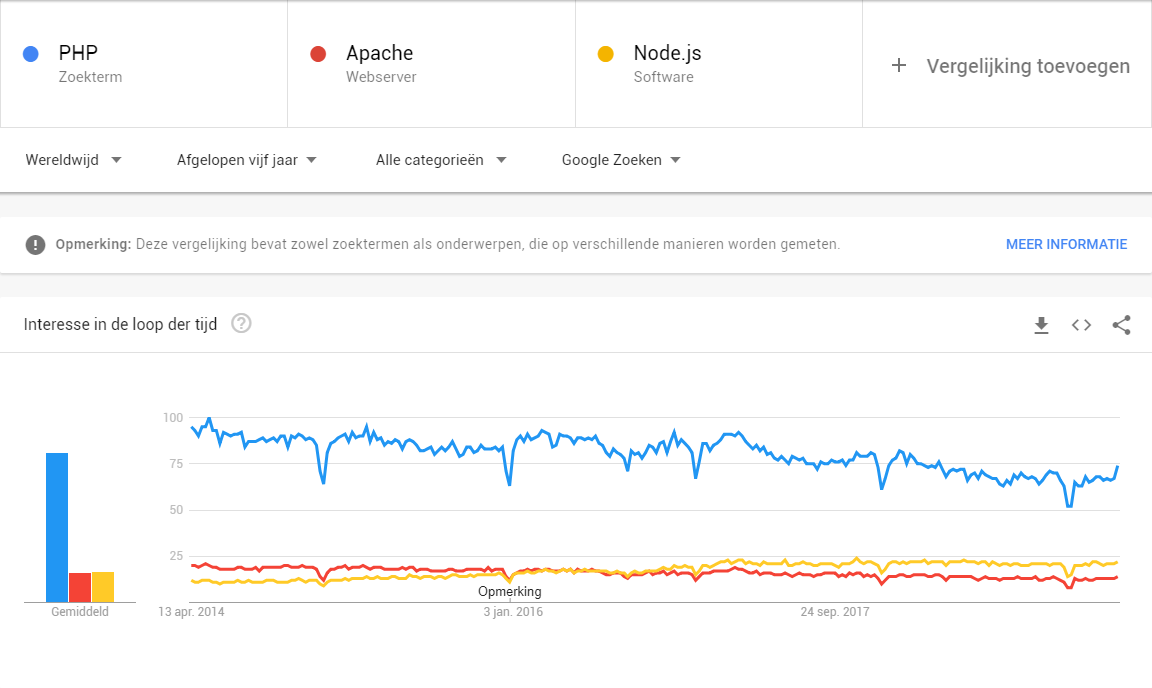
\includegraphics[width=\linewidth]{trend.png}
	\caption{Google searches van PHP (blauw), Apache (rood) en Node.js (geel) in de afgelopen 5 jaar.}
	\label{fig:trend}
\end{figure}

\subsection{Waarom Node.js?}
\label{sec:whyNode}
Node.js is reeds een volwassen server-side framework. Youtube, Yahoo, Google, Amazon, Netflix, Ebay, Reddit, LinkedIn, Paypal, Github, Forbes, Walmart, Uber, NASA, Slack,.. zijn slechts enkele van de duizenden websites die overgeschakeld zijn naar Node.js. En dit zijn geen kleine namen.

Illustrator \textcite{Mehmet2016} toont op een illustratieve wijze de voordelen van Node.js aan. LinkedIn kon hun 15 servers reduceren naar slechts 4 en terwijl de verkeerscapaciteit nog eens verdubbelen. Walmart kon al hun Client-side JavaScript processing naar hun servers verplaatsen, en Ebay kon hun verkeerscapaciteit enorm doen verhogen en hun verbruik enorm doen dalen. De voordelen en functionaliteiten worden hieronder nog eens opgesomd zoals aangegeven door \textcite{Chandrayan2017}.

\subsubsection{Asynchroon}
\label{sec:async}

Node.js is sterk afhankelijk van asynchrone en continue programmeerstijl. I/O-bewerkingen worden uitgevoerd door middel van oproepen naar asynchrone functies waarbij een callback moet worden doorgegeven om aan te geven hoe de berekening wordt voortgezet zodra de genoemde I/O-bewerking asynchroon is voltooid. Het Node.js executiemodel bestaat uit een hoofdgebeurtenislus die wordt uitgevoerd op een single-threaded proces. dankzij deze \textit{event loop} moet een Node.js server nooit wachten op antwoord, het kan gewoon blijven doordraaien na een oproep van een API Call en kan dankzij een notificatiesysteem op een later moment het antwoord terugsturen. Dit maakt Node.js enorm schaalbaar, in tegenstelling tot Apache dat slechts een gelimiteerd aantal threads kan starten om handelingen uit te voeren.

Het is daarom niet altijd makkelijk om deze soort frameworks te debuggen, en het wordt uiteindelijk een uitdagende taak. Gelukkig zijn hiervoor dan ook weer verschillende hulpmiddelen en tools uitgebracht om dit te vereenvoudigen. Zoals hierboven vermeld in ~\autocite{Runtime2017}, kan asynchrone code subtiele bugs opleveren die niet meteen zichtbaar zijn.  Hier is nog niet echt onderzoek over gedaan. Waarin er honderden vergelijkende studies bestaan over de frameworks zelf en of Node.js een goede optie is, zijn er geen of amper studies over de beste manier om dit te debuggen en hoe men dit het best aanpakt. ~\autocite{Runtime2017} vertelt ons meer over het identificeren van schaalbaarheidsproblemen en het aanrijken van mogelijke oplossingen. Ze maken gebruik van parametrische uitdrukkingen voor runtime monitoring van Node.js toepassingen, maar ze geven toe dat dit nog maar de eerste stap is en dat hier nog meer onderzoek naar kan gedaan worden. Hier wordt later in dit onderzoek dieper op ingegaan.

\subsubsection{Performant}
\label{sec:fast}

Google Chrome's JavaScript engine, V8, is bijzonder snel. Dahl heeft dit verder ontwikkeld voor Node.js en dit maakt de framework enorm performant en efficiënt in het uitvoeren van code. Veel sneller dan Python, Ruby of Perl.

\subsubsection{NPM}
\label{sec:npm}

Node.js kent een enorm bloeiende community. Deel van Node is zijn Node Package Manager, ofwel npm, en komt meegeleverd bij de installatie. Via npm kan men uit honderdduizenden pakketjes kiezen voor een JavaScript/Node project makkelijk uit te breiden met extra functionaliteiten in één oogwenk. Dagelijks worden er nieuwe pakketjes toegevoegd aan de packet manager, en is makkelijk één van de redenen waarom Node.js zo populair is, aangezien het ontwikkelen van een webapplicatie enorm vereenvoudigd wordt.   



\section{Express}
\label{sec:express}




 






 

%%=============================================================================
%% Methodologie
%%=============================================================================
\chapter{Methodologie}
\label{ch:methodologie}

%% TODO: Hoe ben je te werk gegaan? Verdeel je onderzoek in grote fasen, en
%% licht in elke fase toe welke stappen je gevolgd hebt. Verantwoord waarom je
%% op deze manier te werk gegaan bent. Je moet kunnen aantonen dat je de best
%% mogelijke manier toegepast hebt om een antwoord te vinden op de
%% onderzoeksvraag.

Nu de vereisten van Kayzr gekend zijn, kan het ontwerpen van de middleware toepassing van start gaan. Hiervoor zal er een bepaalde werkwijze worden gehanteerd, waarover zo dadelijk meer uitleg wordt gegeven. Tijdens het ontwerpen van de middleware zal echter niet enkel met Kayzr's requirements rekening gehouden worden. Het is de bedoeling dat dit geen hardcoded stuk software in Kayzr's backend wordt, maar een abstracte, universele middleware dat gedownload en geïnstalleerd kan worden via Node.js package manager.  

\section{Werkwijze}
\label{sec:werkwijze}

Men is als volgt te werk gegaan: eerst werd een middleware ontwikkeld dat op een mooie manier elke request kon loggen in de console. Erna werd een server aangemaakt op één van de servers van Kayzr, en werd daar Grafana en InfluxDB op geïnstalleerd. Tenslotte werd de middleware geabstraheerd, waarna er getracht werd om connectie te maken met de databank en telkens na een bepaald interval, data naar InfluxDB weg te schrijven. Wanneer de data van de middleware tenslotte Grafana bereikte, werd de middleware geïnstalleerd op Kayzr's backend. Op het einde werden er dan grafieken aangemaakt in Grafana die de requirements van Kayzr zouden volbrengen. 

\subsection{Multilogger}
\label{sec:multilogger}

De te ontwikkelen middleware werd omgedoopt tot Multilogger (en later officieel express-influx-multilogger). Als eerste werd een basis express applicatie aangemaakt, waarin de eerste stapjes middleware software werden geschreven. Als eerste werd er geprobeerd om per keer dat een API call werd gemaakt, de methode van deze call naar de console te loggen.

In app.js
\begin{lstlisting}[language=JavaScript, breaklines=true, numbers=left, frame=single, caption={app.js eerste stap},label=code:appjsFirst]
var app = express();

app.use(bodyParser.json());
app.use(bodyParser.urlencoded({ extended: true }));
app.use(express.static(path.join(__dirname, 'public')));

app.use(multilogger.multilog); // Custom middleware

app.use('/', indexRouter);

app.listen(3000);
\end{lstlisting}

In multilogger.js
\begin{lstlisting}[language=JavaScript, breaklines=true, numbers=left, frame=single, caption={multilogger.js eerste stap},label=code:multilogFirst]
const multilogger = {
	multilog: (req, res, next) => {
	console.log('\n=====- Multilogger v0.1 -=====');
	console.log('--- Basic ---\n');
	
	res.on('finish', () => {
		console.info(`${req.method} --- ${res.statusCode} ---  ${res.statusMessage}  at ${new Date().toLocaleString()}`);
		console.info(`Response-time: ${res.getHeader('X-Response-Time')}`);
		console.info(`URL: ${req.hostname} --- ${req.url}`);
		console.info(`Client: ${req.ip} --- ${req.header('User-Agent')}`);
	});
	

	next();
	},
};

module.exports = multilogger; 
\end{lstlisting}

Dit werd uiteindelijk meer uitgebreid, zodat er een mooi breed overzicht naar de console werd gelogd. Natuurlijk wensen niet alle ontwikkelaars dat er per API all naar de console zou worden gelogd met zeer veel overbodige informatie, aangezien dit kan oplopen van (uiteraard afhankelijk van de software) honderden tot duizenden calls per enkele seconden. Daarom werd er een parameter toegevoegd om deze functionaliteit uit te schakelen, met in het achterhoofd dat de middleware niet enkel zou dienen voor een mooi console-overzicht te geven. Dit was een nice-to-have-functionaliteit voor Kayzr, maar was wel een noodzakelijke eerste stap om op verder te bouwen. Ook werd er een aangepaste \textit{error handler} (stuk code dat fouten afhandelt die zich voortdoen tijdens een API call) geschreven, waardoor ook foutberichten konden gelogd worden.

\begin{lstlisting}[language=JavaScript, breaklines=true, numbers=left, frame=single, caption={Parameters toegevoegd},label=code:multilogparams]
app.use(multilogger.log({ development: false, extended: false }));
\end{lstlisting}

\begin{lstlisting}[language=JavaScript, breaklines=true, numbers=left, frame=single, caption={MultiError.js, de custom error handler},label=code:multiError]
const throwMultilogError = () => {
	return (err, req, res, next) => {
		if (!err) {
			return next();
		}
		res.locals.multiError = {
			errorMessage: err.message,
			errorStack: err.stack
		};
		next();
	};
};

module.exports = throwMultilogError;
\end{lstlisting}

\subsection{Grafana en InfluxDB}
\label{sec:grafanaAndInflux}

Vervolgens moest er een systeem gekozen worden om verzamelde data op te slaan en weer te geven. Dit kan natuurlijk gerealiseerd worden met verschillende databanken en frontend frameworks. Origineel werd er geopteerd om gebruik te maken van MySQL samen met een React.js applicatie om de data te visualiseren, maar na verder onderzoek bleek dat hier reeds handigere software voor bestaat, namelijk InfluxDB, en Grafana, dixit \textcite{Hill2015}. InfluxDB is een snelle, open source time series database, gemaakt om op een snelle manier data zoals metrieken en events op te slaan, gebonden doorheen een tijdsperiode. Grafana daarentegen, is een open platform om time series data om te zetten in prachtige grafieken. Het spreekt dan ook voor zich dat deze twee hand in hand gaan.

Er werd een server van Kayzr toegewezen om dit te testen. Hiervoor werden via Docker twee containers aangemaakt (een soort van virtuele omgeving om deze software op te laten draaien), en werden tenslotte toegewezen aan InfluxDB en Grafana. Uiteindelijk werd de server opgestart, werd Grafana geïnstalleerd en geïnitialiseerd en werd de (lege) Influx-databank gekoppeld. 

\subsection{Wegschrijven en abstraheren}
\label{sec:abstraction}
Nu dat de databank was aangemaakt, werd het tijd om deze te koppelen aan de middleware. Gebaseerd op het voorgaande logsysteem, werd een object aangemaakt dat alle belangrijke info zou bevatten. 

\begin{lstlisting}[language=JavaScript, breaklines=true, numbers=left, frame=single, caption={Log object},label=code:multilogLogObject]
const object = {
	method: req.method,
	statusCode: res.statusCode,
	statusMessage: res.statusMessage,
	date: new Date().toUTCString(),
	responseTime: elapsedTimeInMs,
	contentType: req.header("Content-Type") || " ",
	hostname: req.hostname,
	url: req.url,
	path: res.statusCode !== 404 && req.route && req.route.path ? req.route.path : "No Path",
	body: req.method === "POST" ? realBody : " ",
	params: _.isEmpty(req.params) ? " " : JSON.stringify(req.params),
	query: _.isEmpty(req.query) ? " " : JSON.stringify(req.query),
	cookies: _.isEmpty(req.cookies) ? " " : JSON.stringify(req.cookies),
	auth: req.header("Authorization") || req.header("x-access-token") || " ",
	ip: req.connection.remoteAddress,
	location: location,
	clientInfo: req.header("User-Agent") || " ",
	memoryUsage: memoryUsage,
	cpuUsage: cpuUsage,
	errorMessage: res.locals.multiError || " "
};

\end{lstlisting}

Via een reeds bestaande npm package, namelijk \href{https://github.com/node-influx/node-influx}{\textit{node influx}}, werd dit snel opgelost. Er werd een schema ontwikkeld waaruit optimaal de data zou kunnen geformatteerd worden naar Grafana, en niet veel later vloeiden de eerste metrieken Grafana binnen. Tenslotte werd er een buffer geïmplementeerd, dat om een gegeven interval de opgeslagen data wegschrijft en zichzelf weer leegt voor het volgende interval. 

De volgende stap in het ontwikkelen van een middleware oplossing voor Kayzr, was het abstraheren van de code. Zo kan niet enkel Kayzr hiervan gebruik maken, maar echter iedereen met een Node.js en Express configuratie. Er kwamen wat moeilijkheden opduiken bij het loskoppelen van de code, maar uiteindelijk werd er een abstracte, logische en schaalbare middleware geschreven volgens de richtlijnen van npm. Via parameters kan een gebruiker de functionaliteiten van de middleware aanpassen, en er werd ook ruimte voorzien om later extra database management systemen toe te voegen. De middleware werd omgedoopt tot express-influx-multilogger, werd open source gemaakt en werd uiteindelijk op npm gepubliceerd. Als laatste werd deze gloednieuwe package dan binnengetrokken op de backend en frontend van Kayzr's webplatform. Zo geraakte influx op een snellere manier gevuld met relevante data zodat er begonnen kon worden met het ontwikkelen van de volgende stap. 

\subsection{Grafana's grafieken}
\label{sec:graphs}

Als allerlaatste, werd Grafana opgebouwd om mooie relevante grafieken weer te geven aan de eindgebruiker. De verzamelde data bleek niet altijd even relevant of goed genoeg te zijn om er een grafiek mee op te bouwen, dus was er regelmatig een noodzaak om weer naar de vorige stap terug te gaan en het schema van InfluxDB aan te herzien. Hierdoor kwamen ook nieuwe ideeën tot stand, zoals het toevoegen van een gebruiker zijn geolocatie en het monitoren van de snelheid van elk databank verzoek per API call. Op het moment van schrijven zijn er in Grafana 7 grafieken te bezichtigen.

\subsubsection{Basics}
\label{sec:basics}
Hier worden de basis headers van elke API call getoond. De data bestaat uit een timestamp, ip-adres, response time, host, statuscode, statusbericht, methode, url, pad, en body. 

\begin{figure}[h]
	\centering
	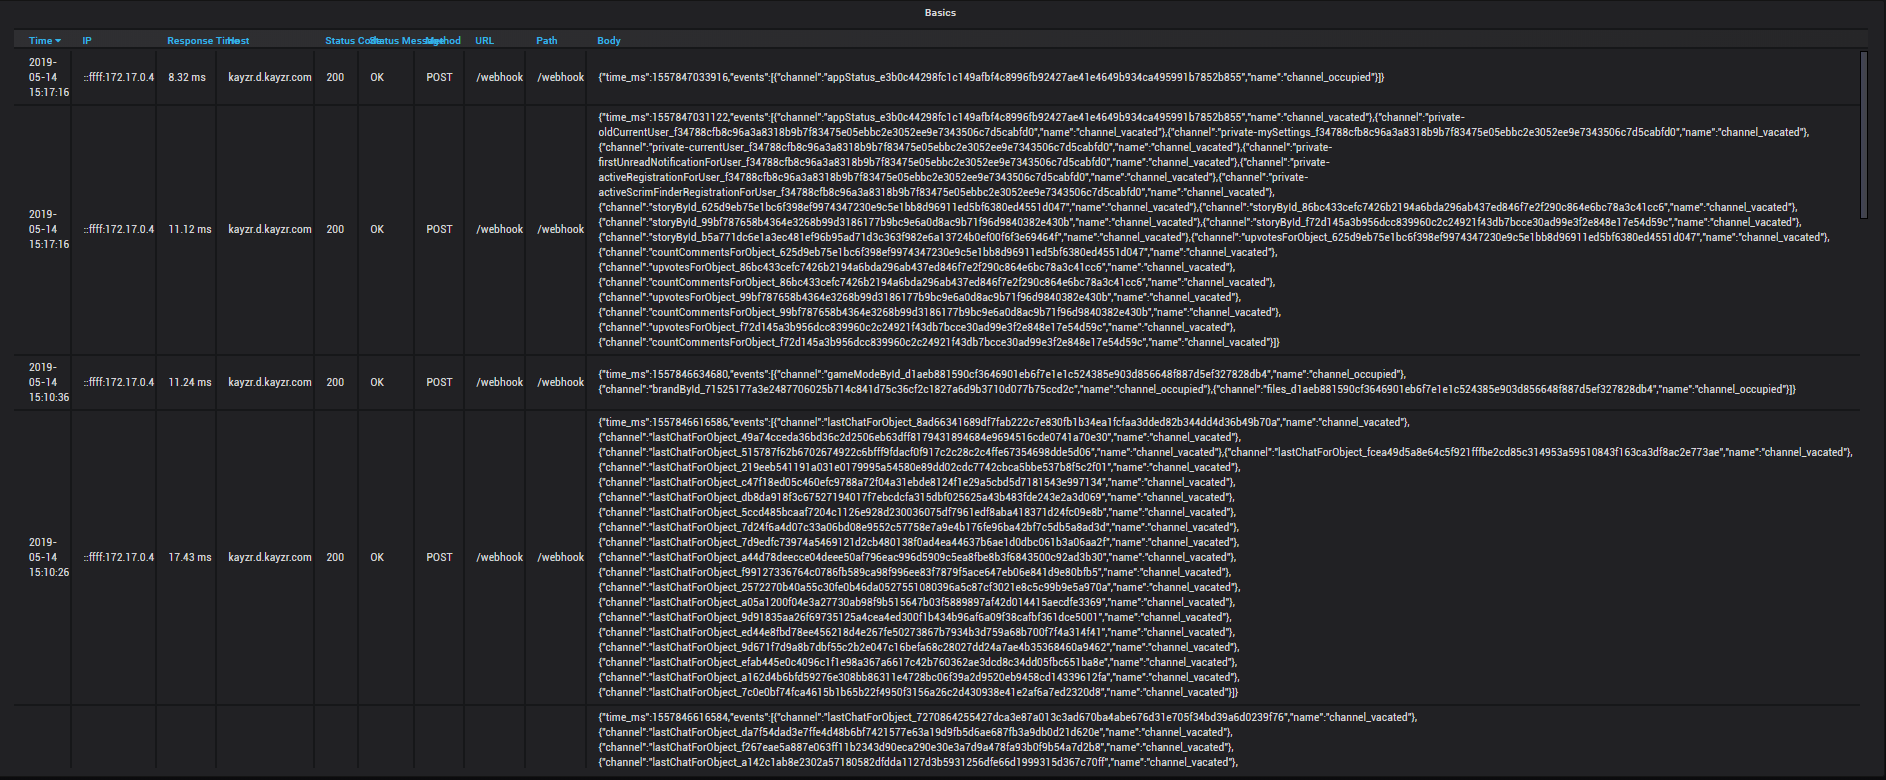
\includegraphics[width=\linewidth]{basics.png}
	\caption{Basics-paneel}
	\label{fig:basics}
\end{figure}

\subsubsection{Number of requests}
\label{sec:numberofrequests}
Het aantal verzoeken in een gegeven tijdsframe. Ook kunnen deze opgesplitst worden per statuscode, zodat men bijvoorbeeld kan observeren hoeveel API calls een fout gaven.

\begin{figure}[h]
	\centering
	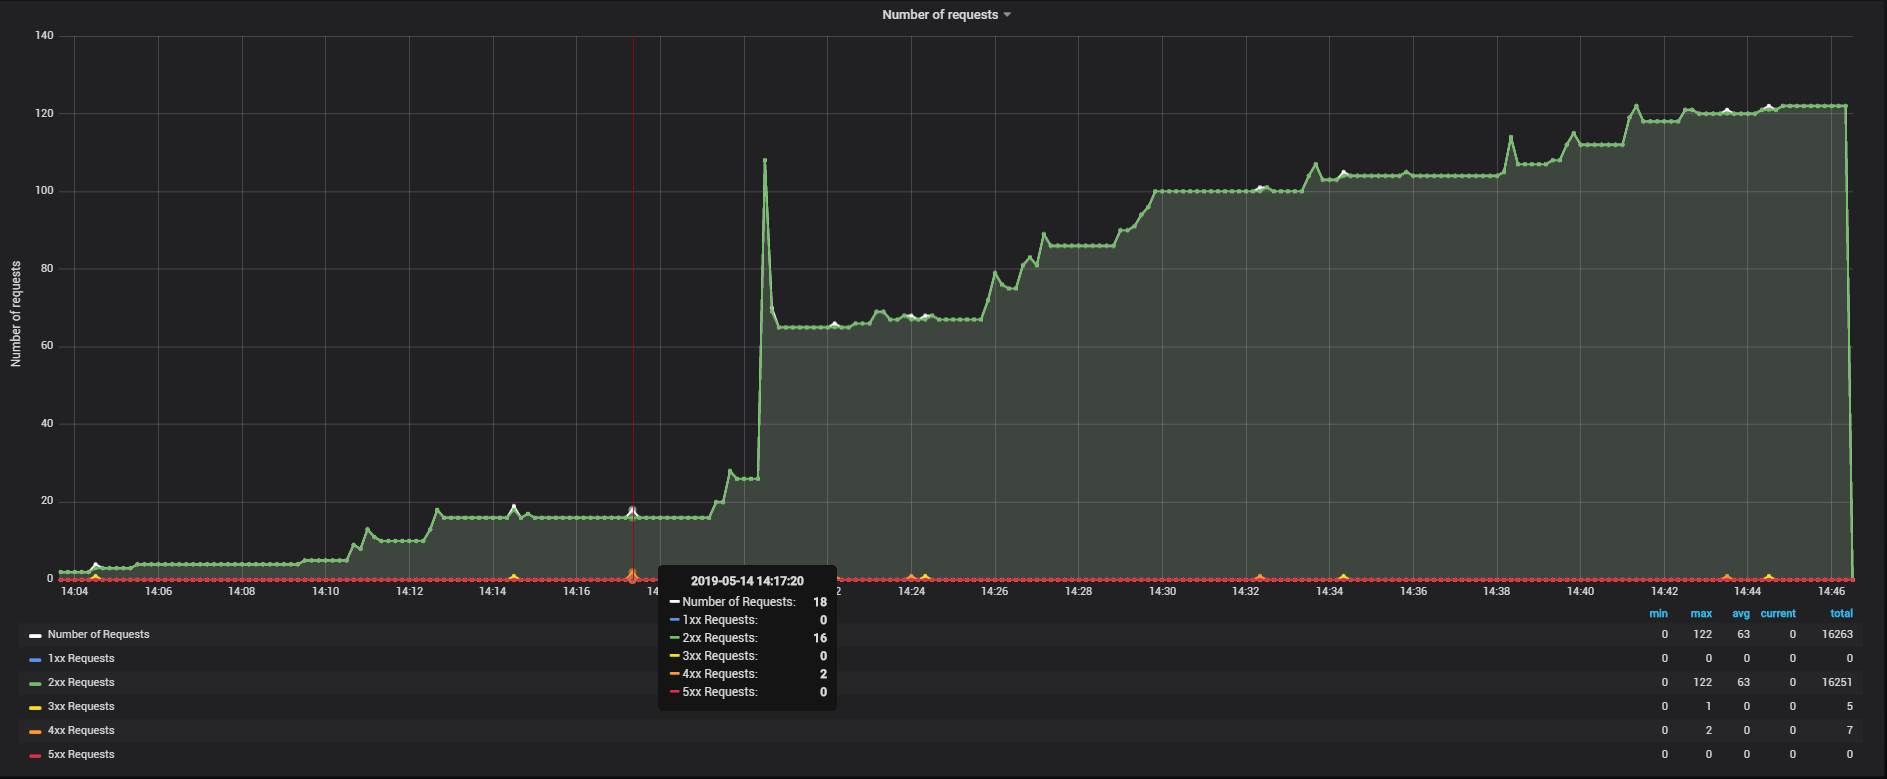
\includegraphics[width=\linewidth]{requests.png}
	\caption{Aantal requests-paneel (wit voor totaal, blauw voor requests dat starten met 1xx, groen voor 2xx, geel voor 3xx, oranje voor 4xx en rood voor 5xx.)}
	\label{fig:requests}
\end{figure}

\subsubsection{Errors}
\label{sec:errors}
Hier worden de foutmeldingen getoond, gegroepeerd per unieke foutmelding. Naast een timestamp, foutmelding en de error stack, worden ook de host, status, url en path weergeven. Aangezien Kayzr dit ook wou gebruiken voor debug-doeleinden, worden ook de body en authenticatietokens weergeven.

\begin{figure}[h]
	\centering
	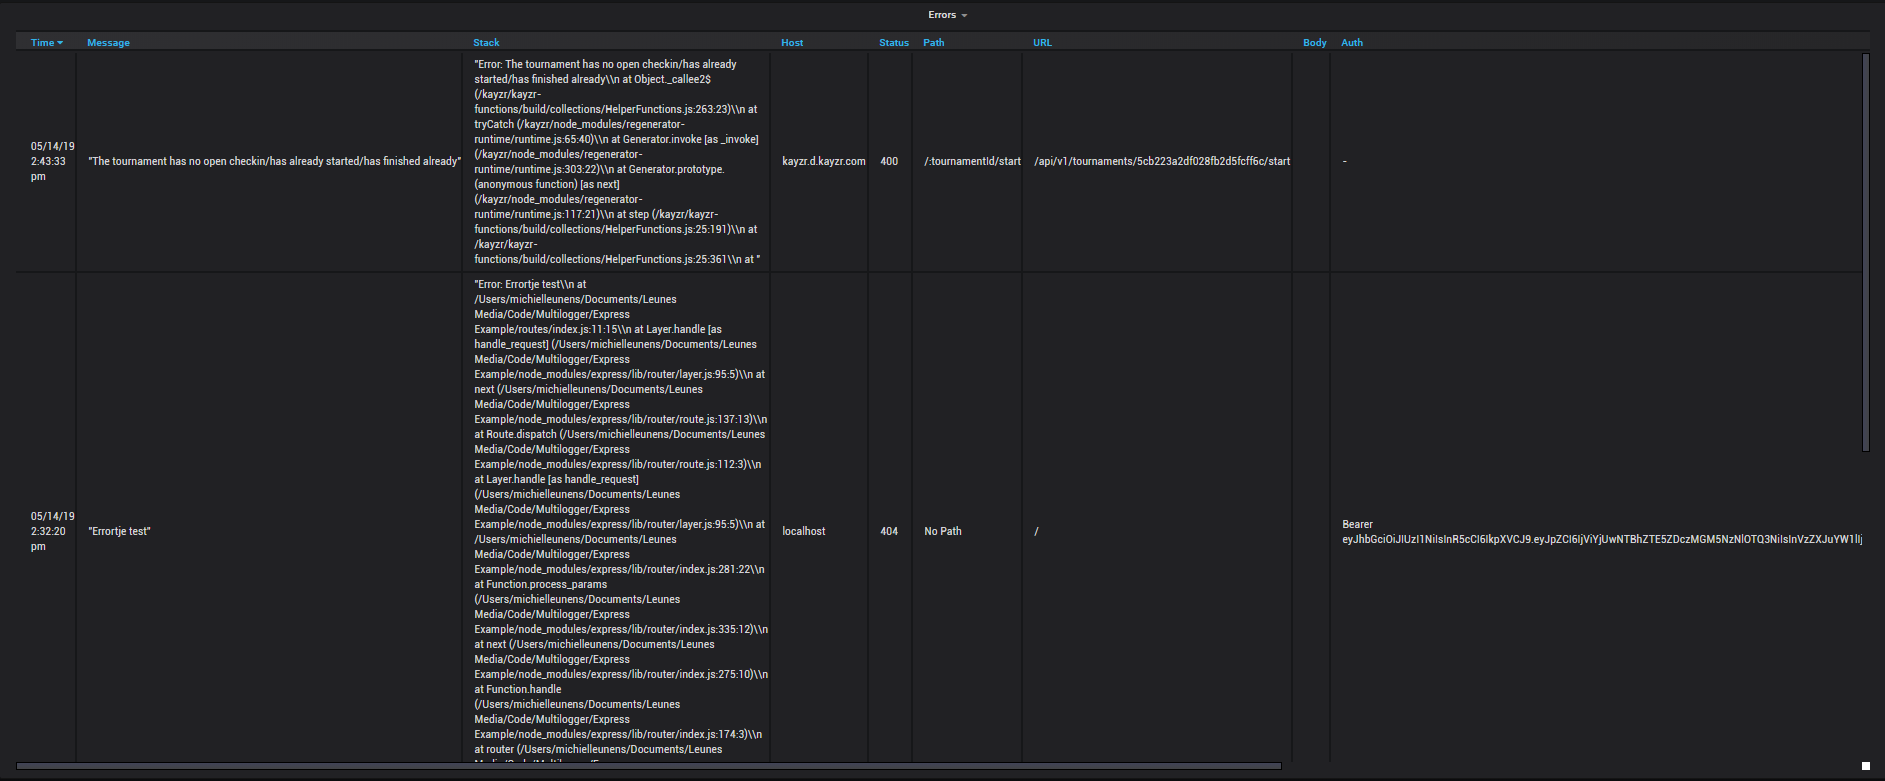
\includegraphics[width=\linewidth]{errors.png}
	\caption{Errors-paneel}
	\label{fig:errors}
\end{figure}

\subsubsection{Database timings}
\label{sec:dbtimings}
Hier wordt per API call de tijden gelogd van een bepaald verzoek naar de databank. Zo kan men per call zien hoeveel tijd het vraag om specifieke data op te halen.

\begin{figure}[h]
	\centering
	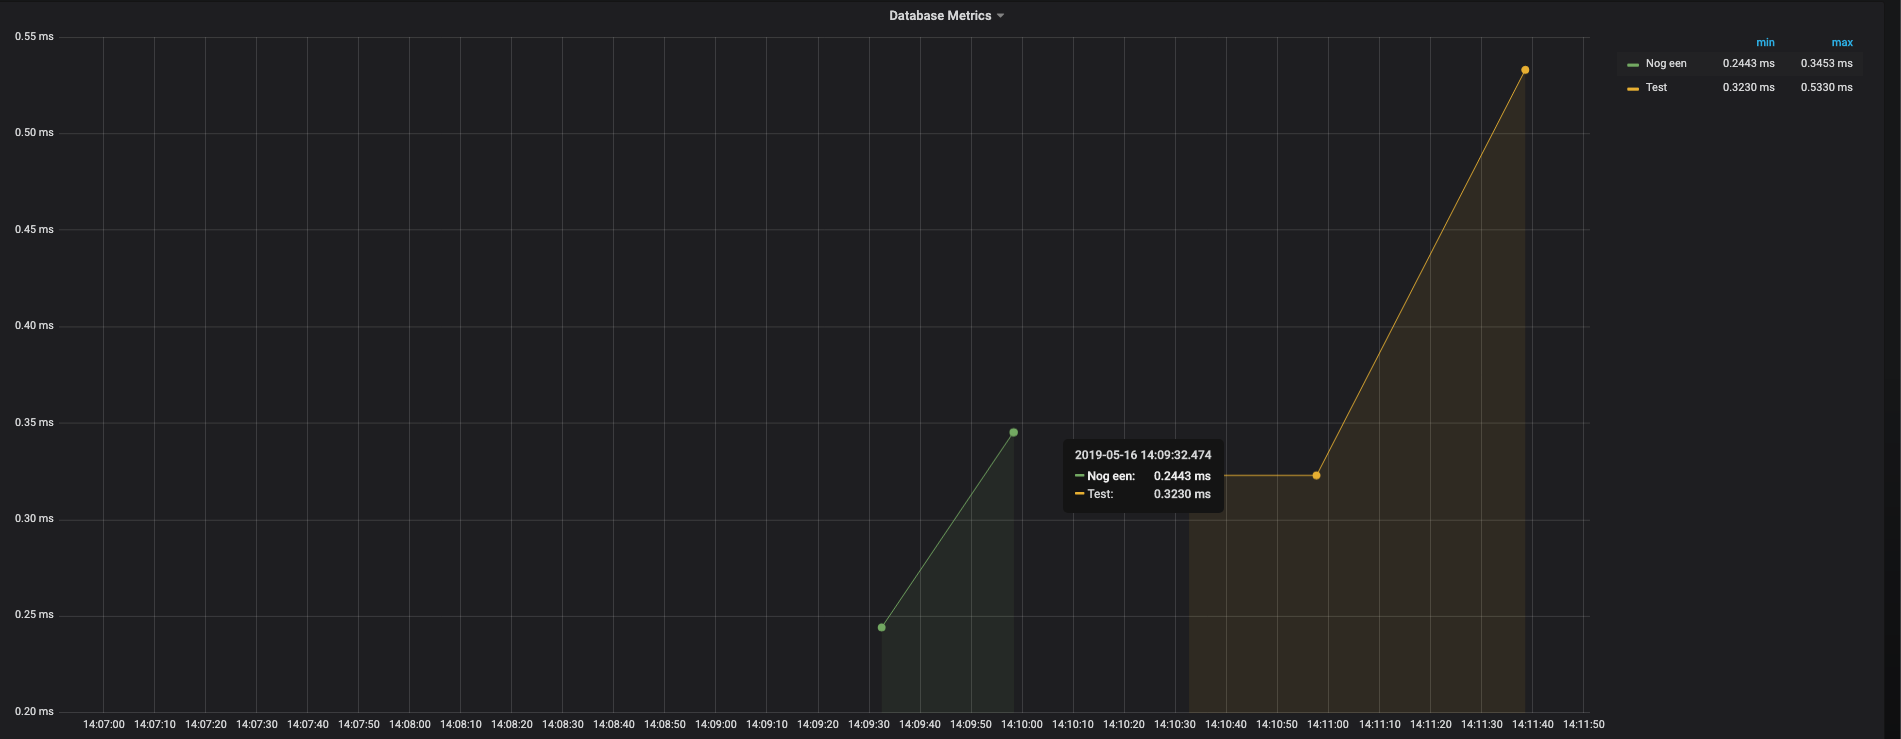
\includegraphics[width=\linewidth]{dbMetrics.png}
	\caption{Database-metrics-paneel}
	\label{fig:dbMetrics}
\end{figure}

\subsubsection{Users}
\label{sec:users}
Op een wereldkaart wordt het aantal gebruikers per land getoond. De geolocatie wordt afgeleid van het ip-adres van de gebruiker, en specifieke locaties worden dus niet opgevraagd.

\begin{figure}[h]
	\centering
	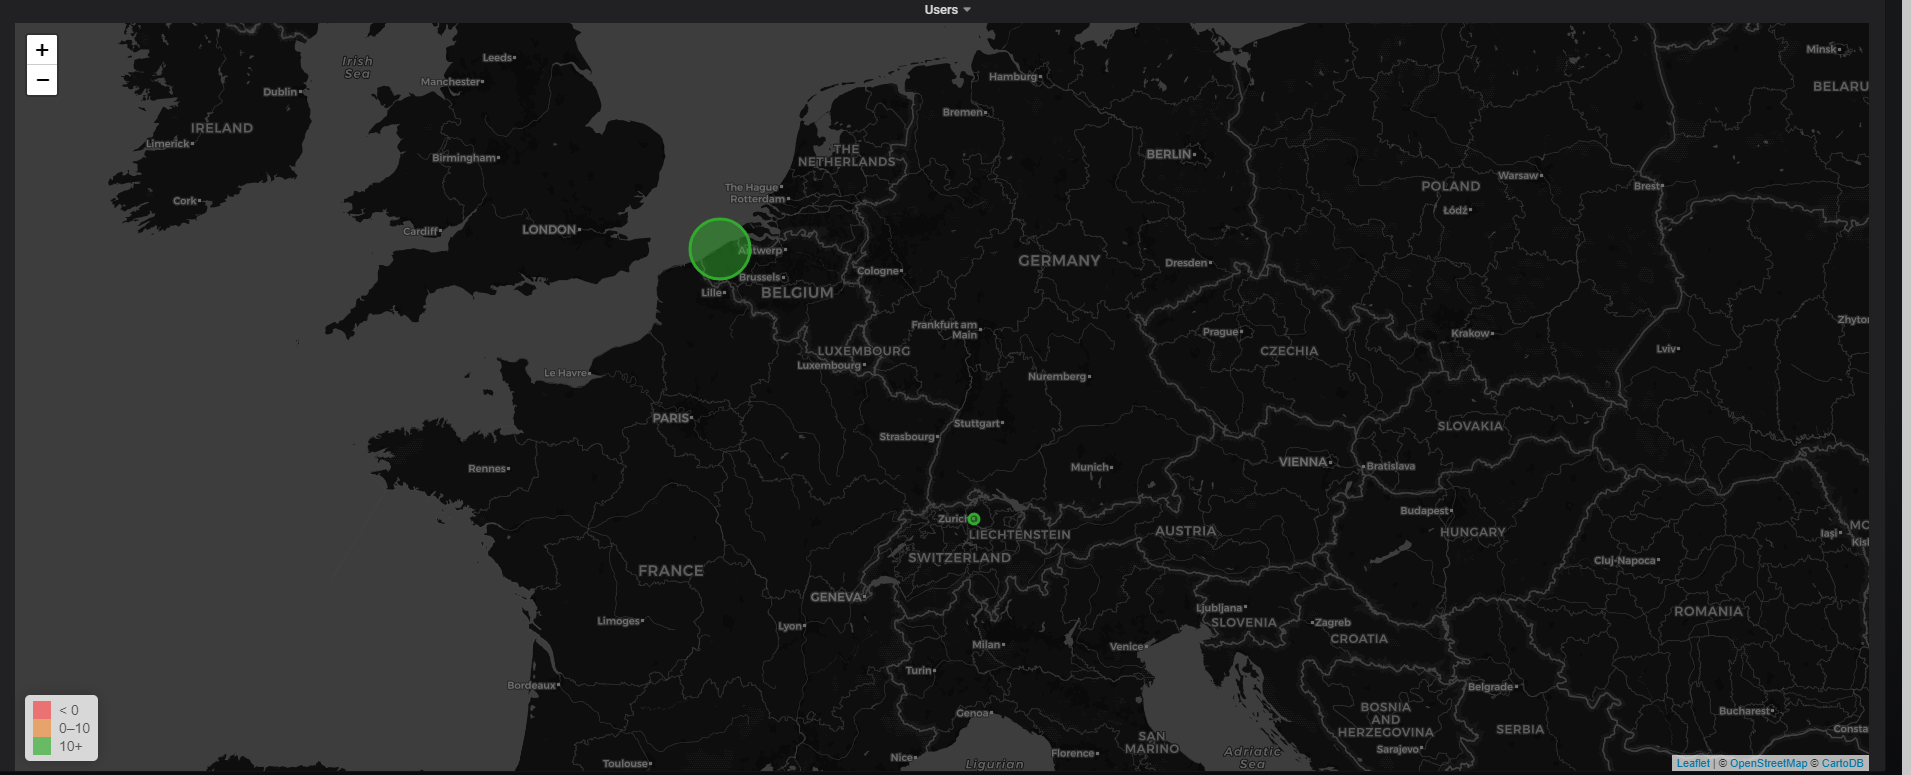
\includegraphics[width=\linewidth]{users.png}
	\caption{Users-paneel}
	\label{fig:users}
\end{figure}

\subsubsection{Memory Usage}
\label{sec:memory}
Het geheugenverbruik per gigabyte van de machine waarop de server draait.
\begin{figure}[h]
	\centering
	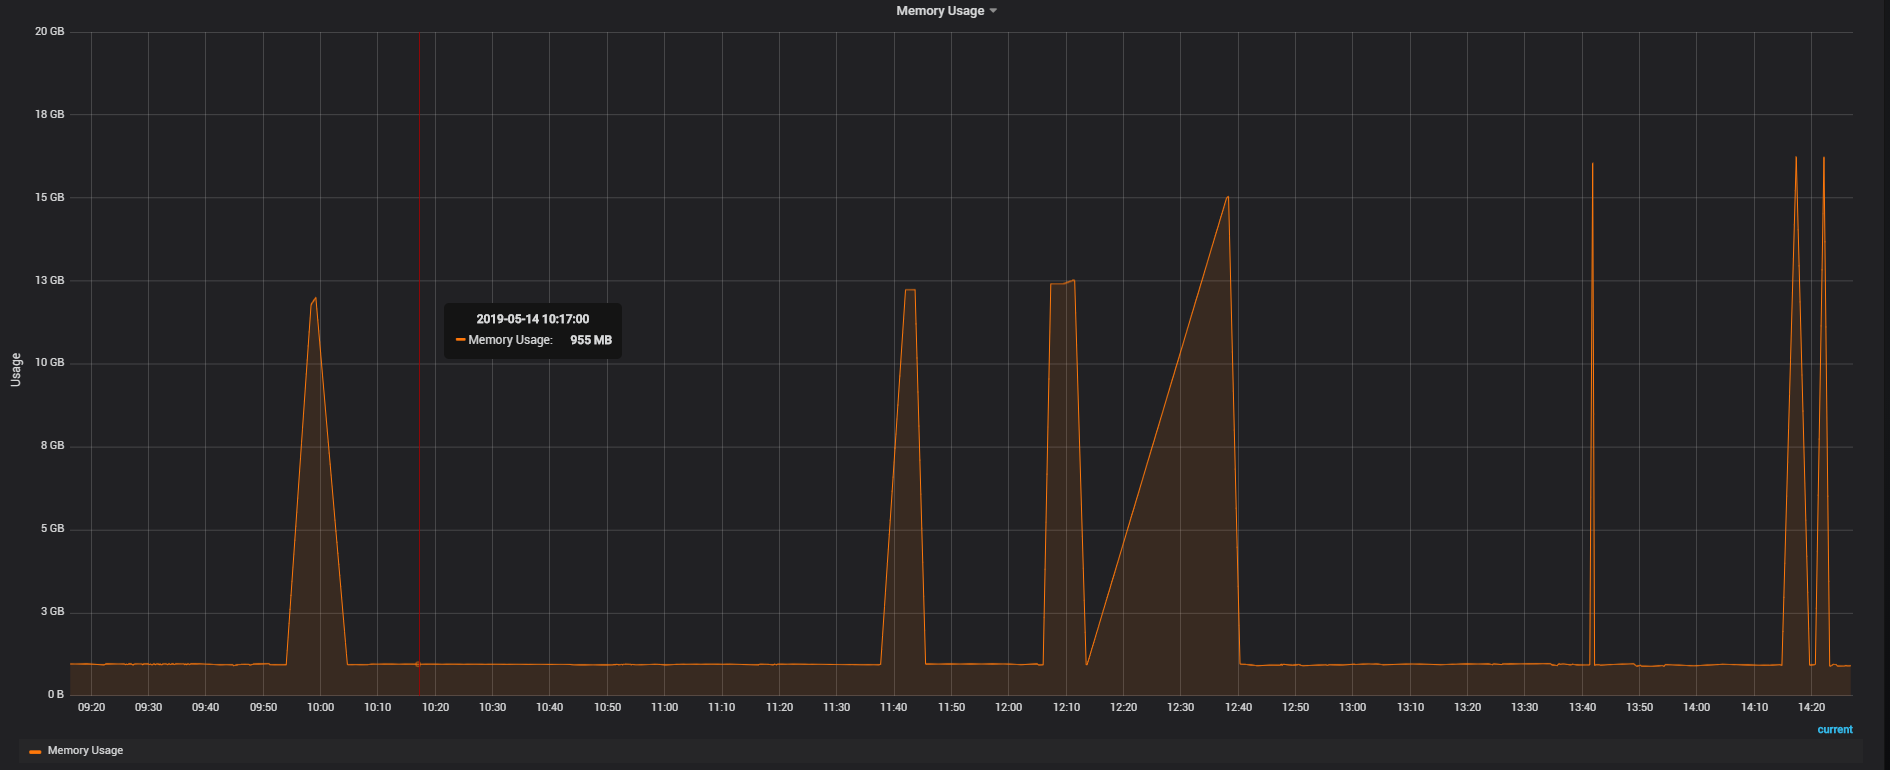
\includegraphics[width=\linewidth]{memory.png}
	\caption{Geheugenverbruik-paneel}
	\label{fig:mem}
\end{figure}

\subsubsection{CPU Usage}
\label{sec:cpu}
Het processorverbruik in percentages van de machine waarop de server draait.

\begin{figure}[h]
	\centering
	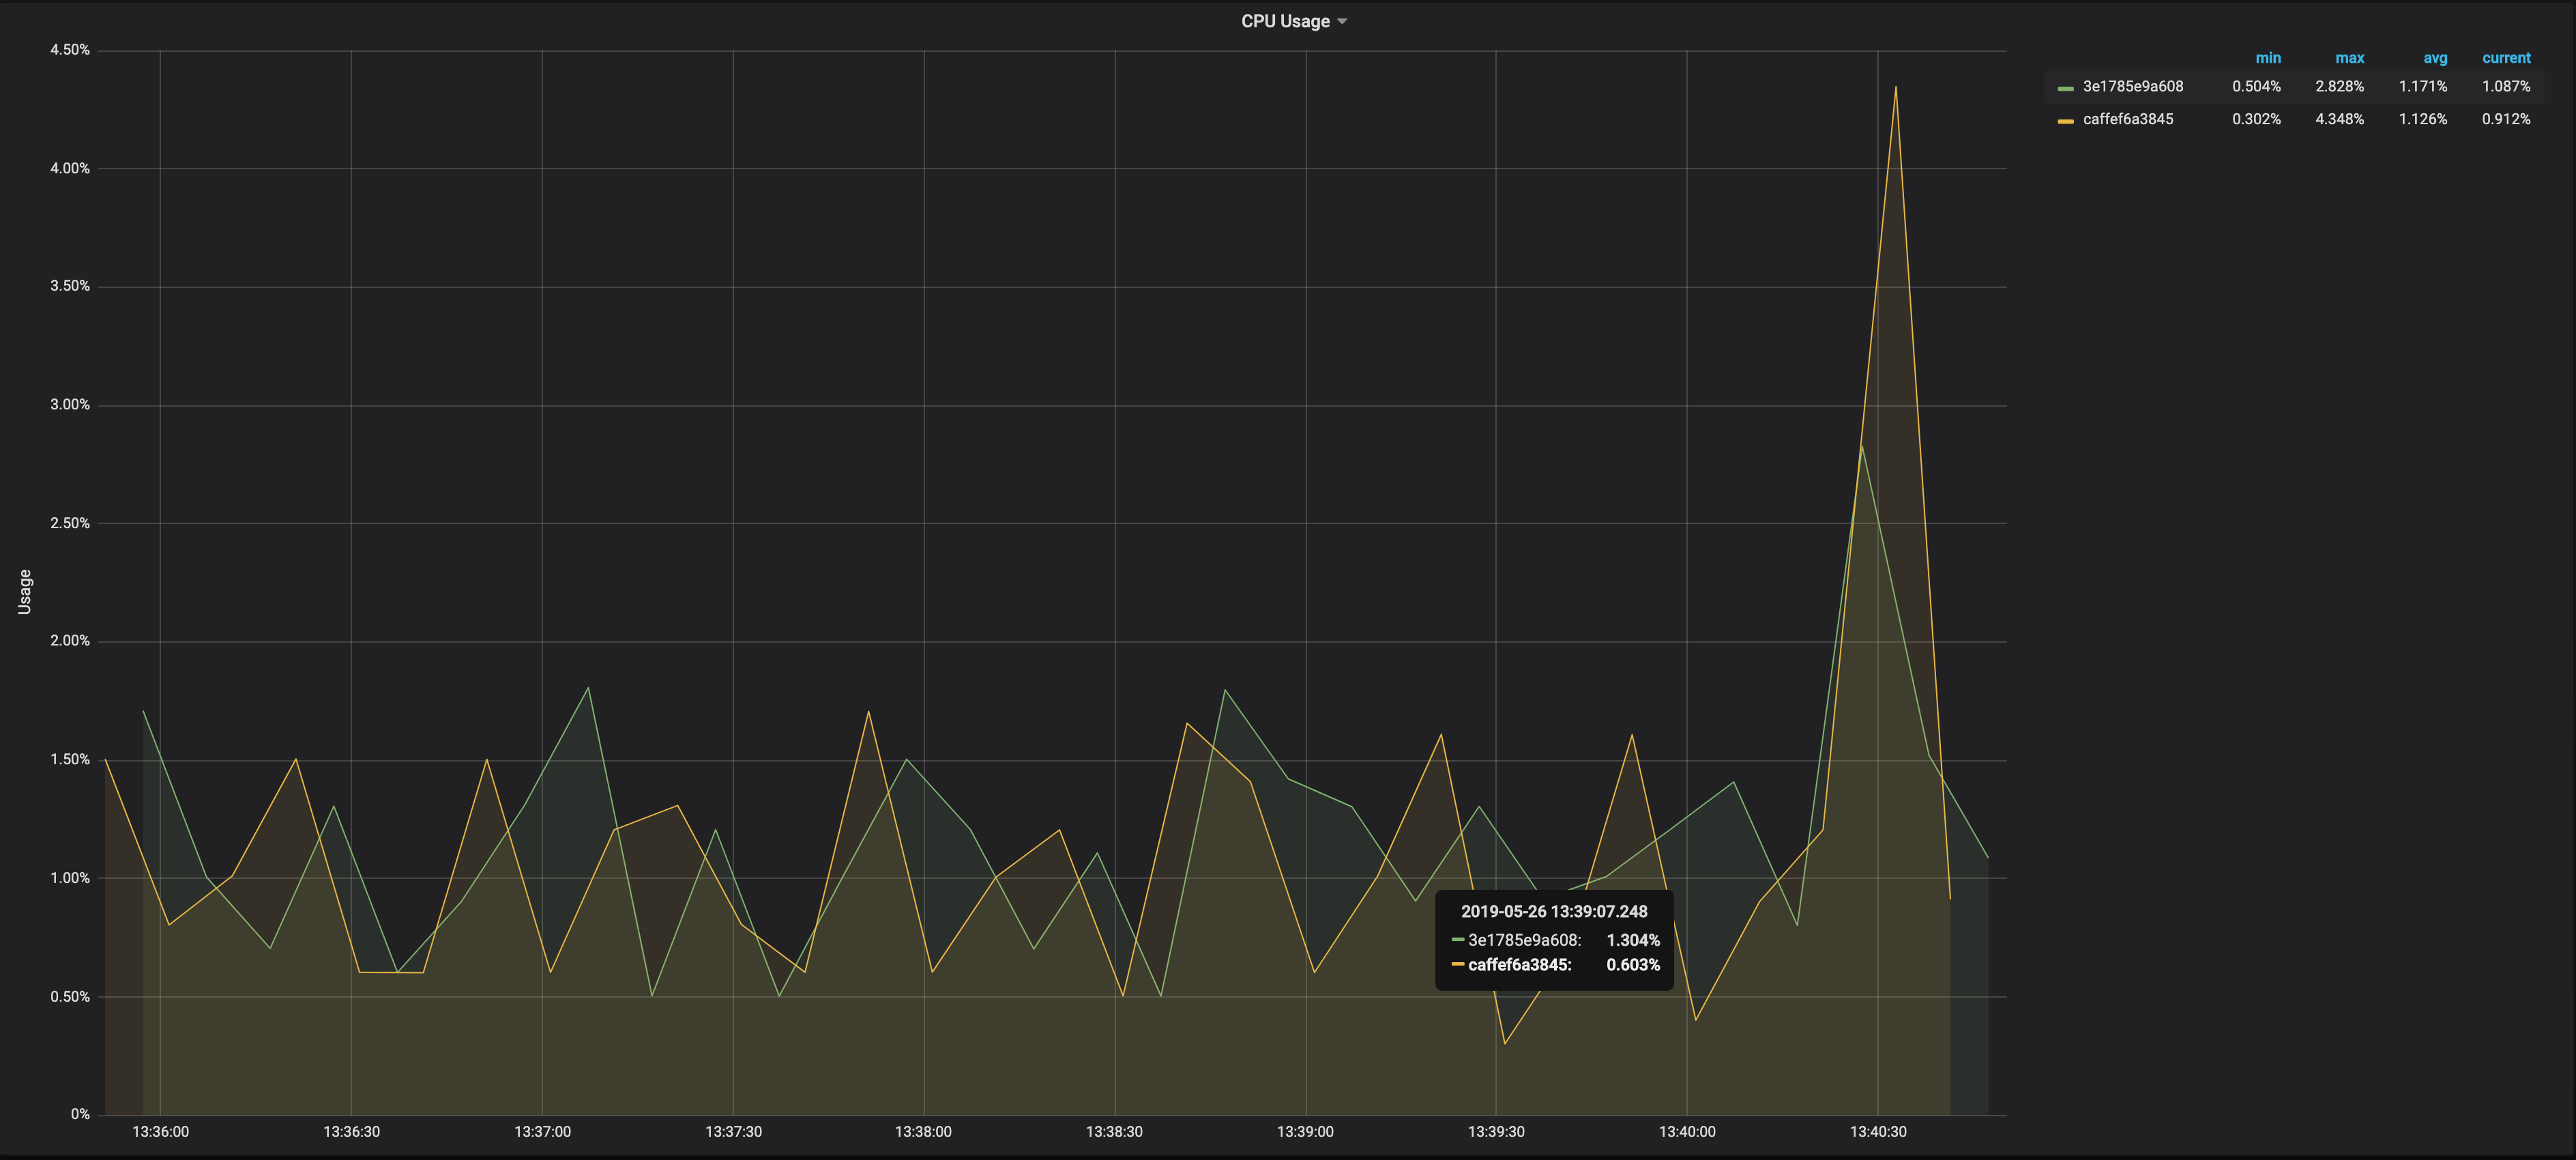
\includegraphics[width=\linewidth]{cpu.png}
	\caption{Processorverbruik-paneel}
	\label{fig:cpu}
\end{figure}

\section{Publicatie}
\label{sec:publication}

De package is ondertussen gepubliceerd op npm onder de naam \href{https://www.npmjs.com/package/express-influx-multilogger}{Express-influx-multilogger,} alsook op \href{https://github.com/LeunensMichiel/express-influx-multilogger}{github}. Installatie en instructies kunnen gevonden worden in de README.md. De middleware is open-source, met het doel om krachtiger en efficiënter te worden in de toekomst toe. Op het moment van schrijven is de laatste versie \textbf{1.0.11}.

\begin{figure}[h]
	\centering
	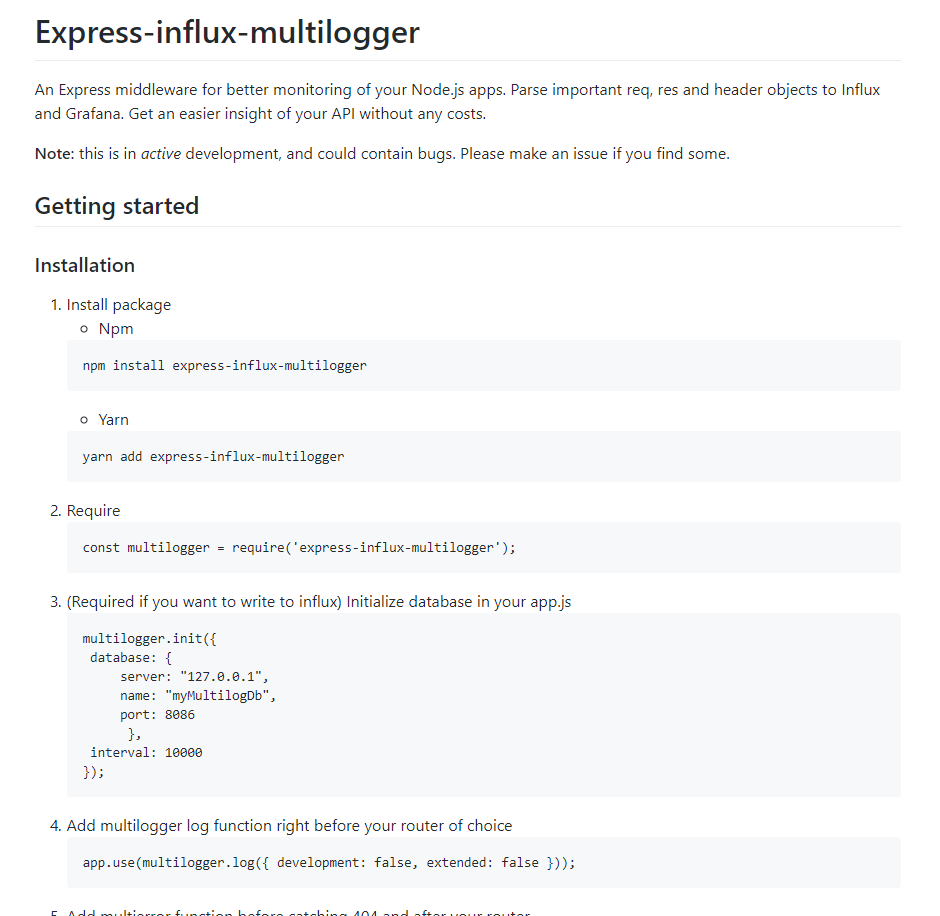
\includegraphics[width=\linewidth]{readme.png}
	\caption{Screenshot van een deel van de README.md. Hier staan onder andere installatie-instructies in, code-voorbeelden, uitleg van de parameters en tal van andere zaken. Wegens incompatibiliteit was het niet mogelijk om de readme weer te geven in LaTeX.}
	\label{fig:readme}
\end{figure}

% Voeg hier je eigen hoofdstukken toe die de ``corpus'' van je bachelorproef
% vormen. De structuur en titels hangen af van je eigen onderzoek. Je kan bv.
% elke fase in je onderzoek in een apart hoofdstuk bespreken.

%\input{...}
%\input{...}
%...

%%=============================================================================
%% Conclusie
%%=============================================================================

\chapter{Conclusie}
\label{ch:conclusie}

%% TODO: Trek een duidelijke conclusie, in de vorm van een antwoord op de
%% onderzoeksvra(a)g(en). Wat was jouw bijdrage aan het onderzoeksdomein en
%% hoe biedt dit meerwaarde aan het vakgebied/doelgroep? Reflecteer kritisch
%% over het resultaat. Had je deze uitkomst verwacht? Zijn er zaken die nog
%% niet duidelijk zijn? Heeft het onderzoek geleid tot nieuwe vragen die
%% uitnodigen tot verder onderzoek?

Nu de middleware is gepubliceerd en binnengetrokken op de servers van Kayzr, kan er worden bekeken of de middleware voldoet aan de vereisten, of er voordelen en al dan niet extra nice-to-haves zijn uit te halen, en of er verbeteringen kunnen plaatsvinden. Dit hoofdstuk zal zich wijden aan het toetsen van de geschreven software aan de praktijk.

\section{Meting aan de vereisten}
\label{sec:reqs}

Vooraleer er een definitieve conclusie wordt gemaakt, moet er eerst gekeken worden of de middleware natuurlijk aan alle opgesomde vereisten voldoet, zoals beschreven in hoofdstuk \ref{sec:requirements}.

\subsection{Toetsing}
\label{sec:testing}

\begin{quote}
	\textit{"Hoeveel keer wordt een bepaalde API call uitgevoerd in een specifieke tijdspanne? Kan Kayzr hierdoor bekijken welke API calls tijdens drukke uren te veel worden opgeroepen en de applicatie vertragen?"}
\end{quote}

Dankzij de \textit{Number of Requests-}tabel, kan dit nu volledig bekeken worden. Men kan kijken hoeveel API calls doorkomen per 10 seconden, of per uur, of per dag,... maar men kan ze ook nog eens groeperen per soort response. Hoeveel 4xx of 5xx calls (calls die foutmeldingen geven) komen door? Ook via de \textit{basics-}tabel kan er veel extra informatie opgevraagd worden. Zo kan met bijvoorbeeld kijken of er tussen 2 pm en 4 pm enkele requests voorkwamen die een uitvoertijd groter dan twintig milliseconden hadden en dus een zware last zouden vormen voor de server. We starten met de eerste vereiste:

\begin{quote}
	\textit{In Google Cloud Stack Driver kan men mooi de errors terugvinden die voorkwamen op de backend server. Maar hier staat nergens de URL van de opgeroepen API call bij. Waar is deze fout beginnen optreden? Kan men die URL verkrijgen opdat men niet moet zoeken naar een naald in een hooiberg?}
\end{quote}

\begin{quote}
	\textit{Kunnen deze fouten ergens opgeslagen worden opdat men later deze fouten makkelijker kan terugvinden?}
\end{quote}


Dit is volledig opgelost. Namelijk door de \textit{errors-}tabel te observeren kan men 
\begin{enumerate}
	\item kijken op welke URL en pad de fout zich voordeed
	\item lezen welke foutmeldingen er werden gegooid, samen met de error stack van de desbetreffende fout.
	\item Ook nuttige parameters aflezen zodat men context kan plaatsen bij de fout. Parameters zoals de request body, authentication token, queries enzovoort.
\end{enumerate}

Fouten kunnen ook opgezocht worden met behulp van een zoekfunctionaliteit, en worden ook geordend volgend error stack en vervolgens volgens error message. Zo worden duplicaten weggefilterd en wordt er een zeer praktisch en gebruikersvriendelijk overzicht weergeven.

\begin{quote}
	\textit{Kan men de (gemiddelde) tijd monitoren tussen het versturen van een bepaalde API call en een verkregen antwoord?}
\end{quote}

De gemiddelde tijd wordt gemonitord en kan in de meeste tabellen teruggevonden worden. Ook is het mogelijk om de gemiddelde tijd van database-calls te monitoren. Hierover wordt later nog eer uitleg gegeven.

\begin{quote}
	\textit{Monitoren van deze Node.js processen hun taxatie op de server waar ze op draaien (CPU, RAM, netwerk,…)}
\end{quote}

Geheugenverbruik en processorverbruik worden per server weergeven in de desbetreffende \textit{performantie-}tabellen.


\begin{quote}
	\textit{Middleware als Morgan toont veel te weinig, Google Cloud Stack Driver toont veel maar geeft geen context mee. De voorgaande opgesomde betalende monitoringsoftware bevatten te veel functies die Kayzr niet meteen zou gebruiken, maar wel handig \textit{zou kunnen} zijn. Dit verantwoordt echter het grote bedrag niet, en Kayzr wenst dus deze som geldt er niet aan te spenderen. Bestaat er geen goede middenweg?}
\end{quote}

Deze tool heeft al bewezen dat deze zeer veel zaken aankan, en schaalbaar is om er meerdere uitbreidingen aan te geven. In de eerste release kan deze al meer dan Morgan, en neemt al de delen die Kayzr handig vindt van Google Cloud Stack Driver over en zet ze om in een eigen Grafana werkomgeving, een werkomgeving die geïmporteerd kan worden in een eigen configuratie waardoor het niet verplicht is om eigen grafieken beginnend van niets op te stellen.

De kost van een Grafana-server voor Kayzr bedraagt ongeveer vijftien euro per maand. Dit is puur voor hosting van een server, en is helemaal geen grote kost. De meeste functionaliteiten van de betalende oplossingen (wiens prijs veel hoger lag, zoals beschreven in \ref{sec:tools}), waren overbodig. Functionaliteiten zoals error stack tracing, konden makkelijk zelf geïmplementeerd worden. En aangezien de middleware open-source en in actieve ontwikkeling is, spreekt het ook voor zich dat in de toekomst meerdere functionaliteiten gaan kunnen toegevoegd worden. Vijftien euro per maand voor één server te laten draaien dat informatie van verschillende servers kan verzamelen, of gemiddeld zeventig euro per maand \textit{per server} voor een veel te uitgebreide tool, kan natuurlijk als een grote overwinning worden beschouwd.

\begin{quote}
	\textit{Afhankelijk zijn van betalende services betekent ook dat Kayzr's data terecht komt bij (dure) third party oplossingen. Is die data veilig? Volgen ze de GDPR regels? Ze hebben liever hun data in eigen handen.}
\end{quote}

Kayzr's data wordt veilig opgeslagen op hun eigen servers. Niemand kan aan die data buiten Kayzr zelf, wat een groot pluspunt is in een tijdsperiode waar privacywetgeving nog nooit zo belangrijk is geacht.

\begin{quote}
	\textit{Men wil niet enkel realtime zaken kunnen bekijken, maar ook data opslaan zodat die op een later moment nog eens bekeken kan worden.}
\end{quote}

InfluxDB is overal beschikbaar op de servers van Kayzr, dus indien de data nog ergens anders moet gebruikt worden, dan kan dit zonder enige moeite.

\subsection{Nice-to-have}
\label{sec:nicetohave}

Verder werden er nog enkele optionele functionaliteiten toegevoegd, en worden hieronder opgesomd. Meerdere extraatjes kunnen mogelijks later worden toegevoegd.

\subsubsection{Geolocatie}
\label{sec:geolocation}

Kayzr kan nu op een interactieve wereldkaart bekijken waar het merendeels van de verzoeken vandaan komen. Er werd geopteerd om de locatie te traceren via een binnenkomend ip-adres. Dit is allesbehalve de meest precieze methode, maar het is meer dan goed genoeg om het land van herkomst af te lezen. Ook wordt er op deze manier geen privacy geschonden van de eindgebruiker. Eindgebruikers die zicht via een vpn-service zouden verbinden mogen worden verwaarloosd, aangezien deze meetpunten relatief weinig voorkomen.

Deze nieuwe functionaliteit is handig om te kijken of een toernooi populairder is in België of Nederland, en of ze misschien kunnen uitbreiden naar het buitenland.

\subsubsection{Databank metrieken}
\label{sec:databaseMetrics}

Sinds versie 1.0.9 is het ook mogelijk om op een willekeurige plek een multilogger-functie op te roepen in je eigen backend. Deze functie heeft de mogelijkheid om een naam, timings en extra parameters mee te krijgen. Zo kan je bijvoorbeeld een specifieke call naar een databank timen (bijvoorbeeld: hoe lang duurt het om een nieuwe gebruiker weg te schrijven naar MySQL). De naam van deze databank en de gemeten tijd stuur je dan mee door, samen met extra optionele parameters. Al deze informatie wordt dan weggewerkt naar InfluxDB en kan dan ook in Grafana worden bekeken. 

\begin{lstlisting}[language=JavaScript, breaklines=true, numbers=left, frame=single, caption={Extra informatie wordt doorgestuurd naar InfluxDB},label=code:addToObject]
const addToObject = ({ name, timing, ...custom } = {}) => {
	let databaseMetrics = {
		name,
		timing
	};
	_.flatMap(custom, param => {
		return _.map(param, (value, key) => {
			return (databaseMetrics[key] = value);
		});
	});
	object.databaseMetrics.push(databaseMetrics);
};
\end{lstlisting}
\begin{lstlisting}[language=JavaScript, breaklines=true, numbers=left, frame=single, caption={Deze functie kan overal in de API worden opgeroepen},label=code:plugin]
router.get("/", function(req, res, next) {
	multilogger.insertDatabaseCallSpeed({
		name: "Testje",
		timing: 5.203,
		custom: {
			optionalInfo: "1",
			2: "3",
			foo: "fighters",
			objectAverageExample: object.example
		}
	});
	res.send("Got a GET request");
	next();
});
\end{lstlisting}


\section{Kayzr's blik op de toekomst}
\label{sec:future}

%Het vermelden dat Kayzr er tevreden mee is, heeft zeker een meerwaarde. Toelichten hoe ze dit gaan gebruiken dan, en wat de next steps voor hen zijn zou ik er wel inzetten dan. 

\section{Uitbreiding en verder onderzoek}
\label{sec:expansin}

%Lessons Learned

%Verder kan je zelf nog aangeven hoe je de middleware kan uitbreiden/verbeteren.

%%=============================================================================
%% Bijlagen
%%=============================================================================

\appendix

%%---------- Onderzoeksvoorstel -----------------------------------------------

\chapter{Onderzoeksvoorstel}

Het onderwerp van deze bachelorproef is gebaseerd op een onderzoeksvoorstel dat vooraf werd beoordeeld door de promotor. Dat voorstel is opgenomen in deze bijlage.

% Verwijzing naar het bestand met de inhoud van het onderzoeksvoorstel
% !TeX spellcheck = de_DE
%---------- Inleiding ---------------------------------------------------------

\section{Introductie} % The \section*{} command stops section numbering
\label{sec:introductie}

NodeJS is een Javascript framework wiens populariteit in de afgelopen jaar hard is toegenomen. Ontwikkelaars genieten van verschillende voordelen. Het werkt asynchroon, het is makkelijk schaalbaar en het is zeer portabel. Doordat het Javascript is, kan elk besturingssysteem gebruik maken van de krachtige backendfuncties van NodeJS. Dit maakt het een uitstekend framework voor webapplicaties te ontwikkelen.  NodeJS is echter niet makkelijk om te monitoren doordat het asynchroon is opgebouwd. Het toepassen van de juiste technieken om te monitoren kan de slaagkansen van een project echter goed verhogen, net als de levenscyclus van de applicatie. Op welke manieren kunnen we het monitoren van zulke applicaties aanpakken? Welke software en tools worden hiervoor gebruikt? Welke technieken worden het best toegepast? En kan er ook intern in het proces van NodeJS gekeken worden en deze informatie toegepast worden? En zijn al deze technieken drastisch veranderd sinds het framework werd uitgebracht in maart 2009? 

%---------- Stand van zaken ---------------------------------------------------

\section{State-of-the-art}
\label{sec:state-of-the-art}



Hier beschrijf je de \emph{state-of-the-art} rondom je gekozen onderzoeksdomein. Dit kan bijvoorbeeld een literatuurstudie zijn. Je mag de titel van deze sectie ook aanpassen (literatuurstudie, stand van zaken, enz.). Zijn er al gelijkaardige onderzoeken gevoerd? Wat concluderen ze? Wat is het verschil met jouw onderzoek? Wat is de relevantie met jouw onderzoek?

Verwijs bij elke introductie van een term of bewering over het domein naar de vakliteratuur, bijvoorbeeld~\autocite{Doll1954}! Denk zeker goed na welke werken je refereert en waarom.

% Voor literatuurverwijzingen zijn er twee belangrijke commando's:
% \autocite{KEY} => (Auteur, jaartal) Gebruik dit als de naam van de auteur
%   geen onderdeel is van de zin.
% \textcite{KEY} => Auteur (jaartal)  Gebruik dit als de auteursnaam wel een
%   functie heeft in de zin (bv. ``Uit onderzoek door Doll & Hill (1954) bleek
%   ...'')


%---------- Methodologie ------------------------------------------------------
\section{Methodologie}
\label{sec:methodologie}

Onderzoek doen naar de verschillende mogelijkheden van software en tools. Een steekproef maken van een aantal node-developers en via een enquete vragen met welke tools zij hun NodeJS applicatie monitoren, uitgebracht tussen 2009 en 2019. We kunnen erna kijken welke tools beter performeren dan anderen dankzij het gebruik van de servers van Kayzr. We kunnen dit uitgebreider onderzoeken door:

\begin{itemize}
	\item Monitoren van api calls volgens het aantal keren opgeroepen
	\item Monitoren van api calls volens duratie tot een response gestuurd wordt
	\item Het gemak om errors op te slaan en later te debuggen/analyseren
	\item Monitoren van deze node process en hun taxatie op de server waar ze draaien (CPU, RAM, netwerk, …)
\end{itemize}

Hier beschrijf je hoe je van plan bent het onderzoek te voeren. Welke onderzoekstechniek ga je toepassen om elk van je onderzoeksvragen te beantwoorden? Gebruik je hiervoor experimenten, vragenlijsten, simulaties? Je beschrijft ook al welke tools je denkt hiervoor te gebruiken of te ontwikkelen. 

%---------- Verwachte resultaten ----------------------------------------------
\section{Verwachte resultaten}
\label{sec:verwachte_resultaten}

Er zal waarschijnlijk wel een tool uitspringen die op alle vlakken gemiddeld goed performeert. Dit zal wel de tool zijn die het meest populair is idk

Hier beschrijf je welke resultaten je verwacht. Als je metingen en simulaties uitvoert, kan je hier al mock-ups maken van de grafieken samen met de verwachte conclusies. Benoem zeker al je assen en de stukken van de grafiek die je gaat gebruiken. Dit zorgt ervoor dat je concreet weet hoe je je data gaat moeten structureren.

%---------- Verwachte conclusies ----------------------------------------------
\section{Verwachte conclusies}
\label{sec:verwachte_conclusies}

De wereld van Javascript is nog in volle groei, maar is toch al een pak matuurder dan vroeger. We zien dat de tools beter zijn geworden. De concurrentie is enorm groot aangezien NodeJS een enorm populair platform is. Daardoor zal het noodzakelijk zijn om een gepaste monitoringtechniek toe te passen adhv software die we reeds kennen en vertrouwen. 

Hier beschrijf je wat je verwacht uit je onderzoek, met de motivatie waarom. Het is \textbf{niet} erg indien uit je onderzoek andere resultaten en conclusies vloeien dan dat je hier beschrijft: het is dan juist interessant om te onderzoeken waarom jouw hypothesen niet overeenkomen met de resultaten.



%%---------- Andere bijlagen --------------------------------------------------
% TODO: Voeg hier eventuele andere bijlagen toe
%\input{...}

%%---------- Referentielijst --------------------------------------------------

\printbibliography[heading=bibintoc]
%\addcontentsline{toc}{chapter}{\textcolor{maincolor}{\IfLanguageName{dutch}{Bibliografie}{Bibliography}}}

\end{document}
